\documentclass[usenames,dvipsnames,11pt,pdf,utf8,russian,aspectratio=43]{beamer}
\usepackage{cmap}
\usepackage[T2A]{fontenc}
\usepackage[english,russian]{babel}
\usepackage{subfig}
\usepackage{color}
\usepackage{multicol}
\usepackage{appendixnumberbeamer}
\usepackage{multicol}
\usepackage{tikz}
\usepackage{mathbbol}
\usepackage{amssymb}             % AMS Math

\DeclareSymbolFontAlphabet{\mathbb}{AMSb}%
\DeclareSymbolFontAlphabet{\amsmathbb}{bbold}%


\usetikzlibrary{arrows,automata}
\usetikzlibrary{positioning}



\DeclareMathOperator*{\argmin}{arg\,min}

\DeclareMathOperator*{\argmax}{arg\,max}
%
% Choose how your presentation looks.
%
% For more themes, color themes and font themes, see:
% http://deic.uab.es/~iblanes/beamer_gallery/index_by_theme.html
%
\mode<presentation>
{
  \usetheme{Boadilla}      % or try Darmstadt, Madrid, Warsaw, ...
  \usecolortheme{seagull} % or try albatross, beaver, crane, ..

  \usefonttheme{structurebold}  % or try serif, structurebold, ...
  \setbeamertemplate{navigation symbols}{}
  \setbeamertemplate{caption}[numbered]

} 
\setbeamercolor{mygray}{fg=gray,bg=white}


\setbeamertemplate{footline}
{
  \leavevmode%
  \hbox{%
  \begin{beamercolorbox}[wd=.9\paperwidth,ht=2.25ex,dp=1ex,center]{}%
   
  \end{beamercolorbox}%
  \begin{beamercolorbox}[wd=.1\paperwidth,ht=2.25ex,dp=1ex]{mygray}%
   
    \insertframenumber{} / \inserttotalframenumber\hspace*{1ex}
  \end{beamercolorbox}}%
  \vskip0pt%
}



\captionsetup[subfloat]{labelformat=empty}
\title[Выбор структуры модели]{Байесовский выбор\\ субоптимальной структуры\\ модели глубокого обучения}
\author{О.\,Ю.\,Бахтеев}


\institute[]{Диссертация на соискание ученой степени\\
кандидата физико-математических наук\\05.13.17 --- Теоретические основы информатики\\Научный руководитель: д.ф.-м.н. В.В. Стрижов\\}     
%\institute[МФТИ]{Московский Физико-Технический Институт (Государственный Университет)}
\date[2019]{Московский физико-технический институт\\5 июня 2019 г.}
\begin{document}

\begin{frame}
  \titlepage
\end{frame}



\begin{frame}{Выбор  структуры модели глубокого обучения}
\small
\textbf{Цель: } предложить метод выбора структуры модели глубокого обучения.\\
\textbf{Задачи}
\begin{enumerate}
\item Предложить критерии оптимальной и субоптимальной сложности модели глубокого обучения.
\item Предложить алгоритм построения модели субоптимальной сложности и оптимизации параметров.
\end{enumerate}
\textbf{Исследуемые проблемы}
\begin{enumerate}
\item Большое число параметров и гиперпараметров модели, высокая вычислительная сложность оптимизации.
\item Многоэкстремальность и невыпуклость задачи оптимизации.
\end{enumerate}
\textbf{Методы исследования}\\ 
Рассматриваются графовое представление нейронной сети. Используются методы вариационного байесовского вывода.  Для получения модели субоптимальной сложности используется метод автоматического определения релевантности параметров с использоваением градиентных методов оптимизации гиперпараметров и структурных параметров модели.
\end{frame}



\begin{frame}    
                                                                                                                        
\frametitle{Проблема выбора оптимальной структуры }                                                                                                          
Правдоподобие моделей с избыточным числом параметров значимо не меняется при их удалении.                                                       
\begin{figure}[h]                                                                                                                               
\centering                                                                                                                                      
\subfloat[Избыточность параметров модели]{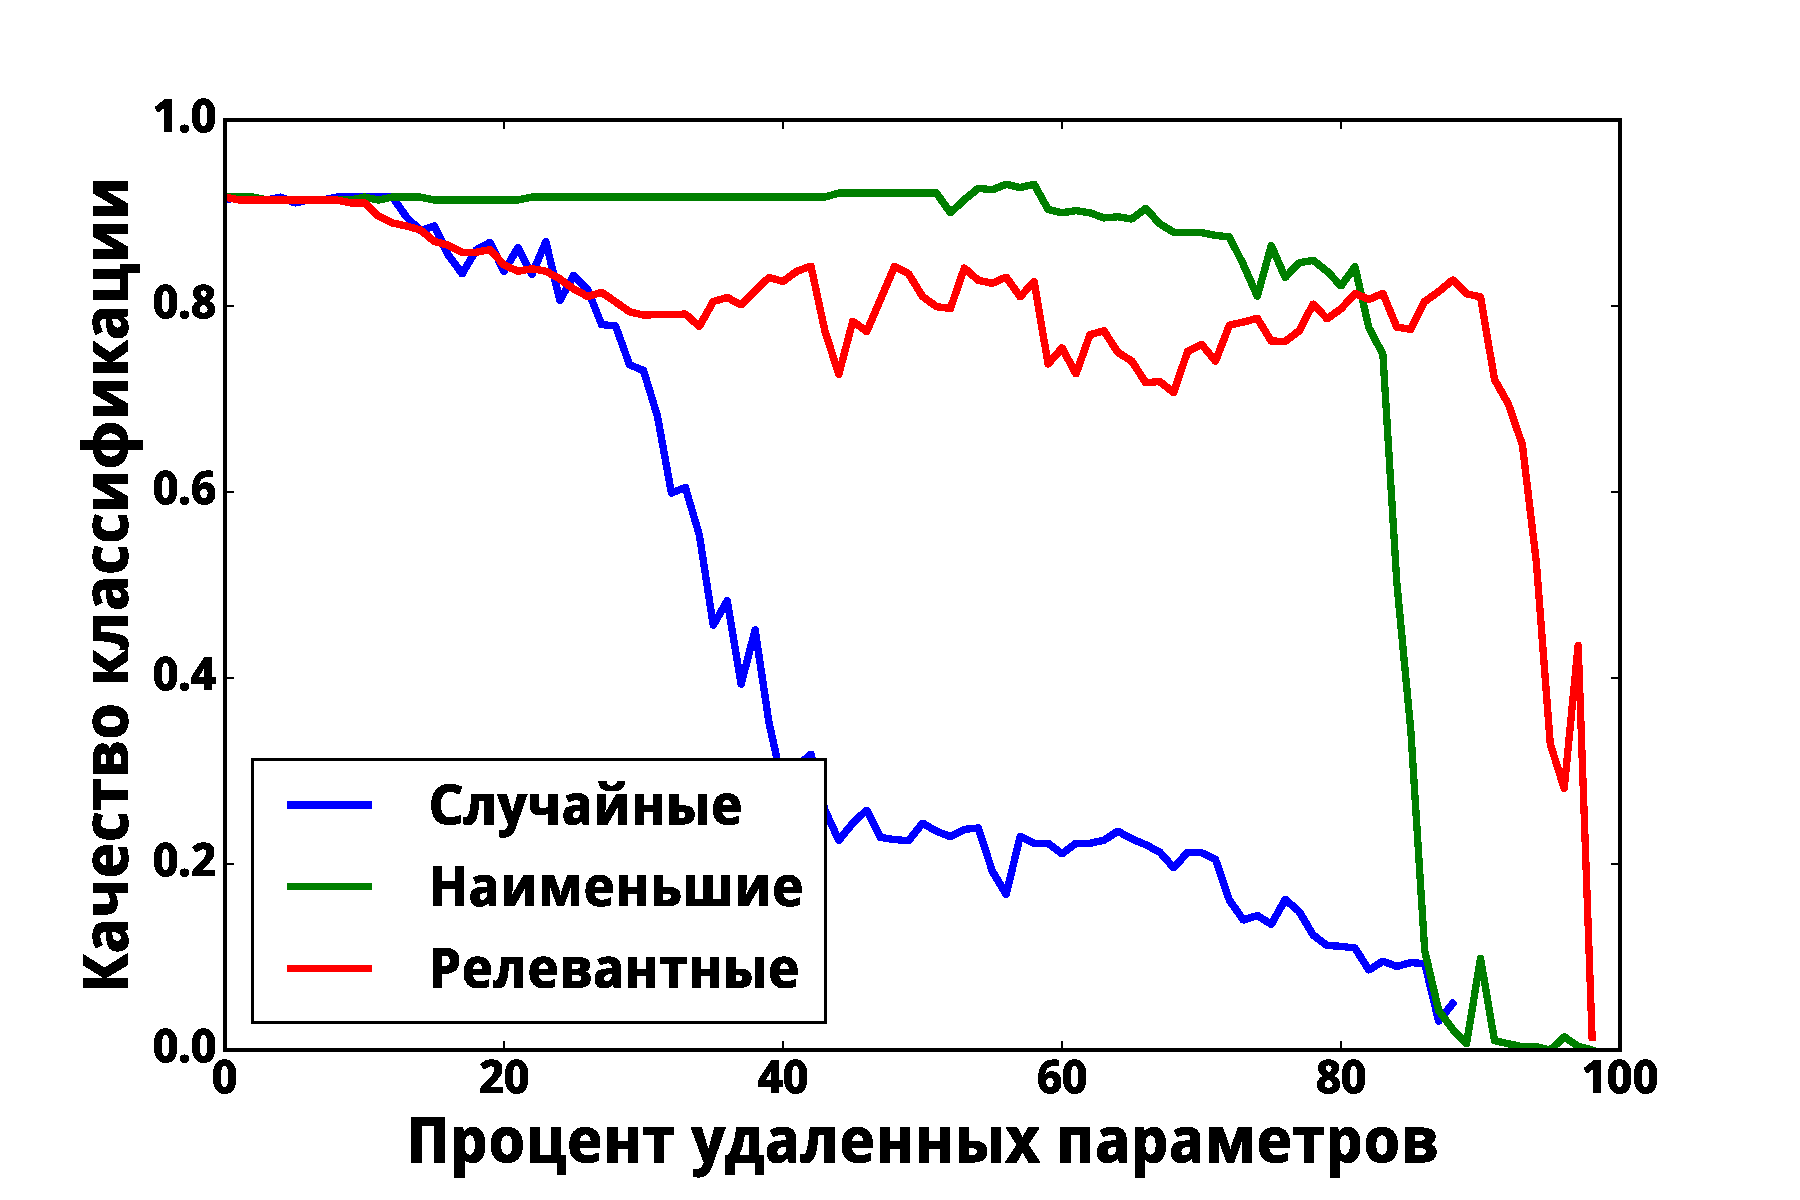
\includegraphics[width=0.55\textwidth]{./slide_plots/pruning.pdf}}   
\hspace*{-1cm}                                       
\subfloat[Устойчивость модели]{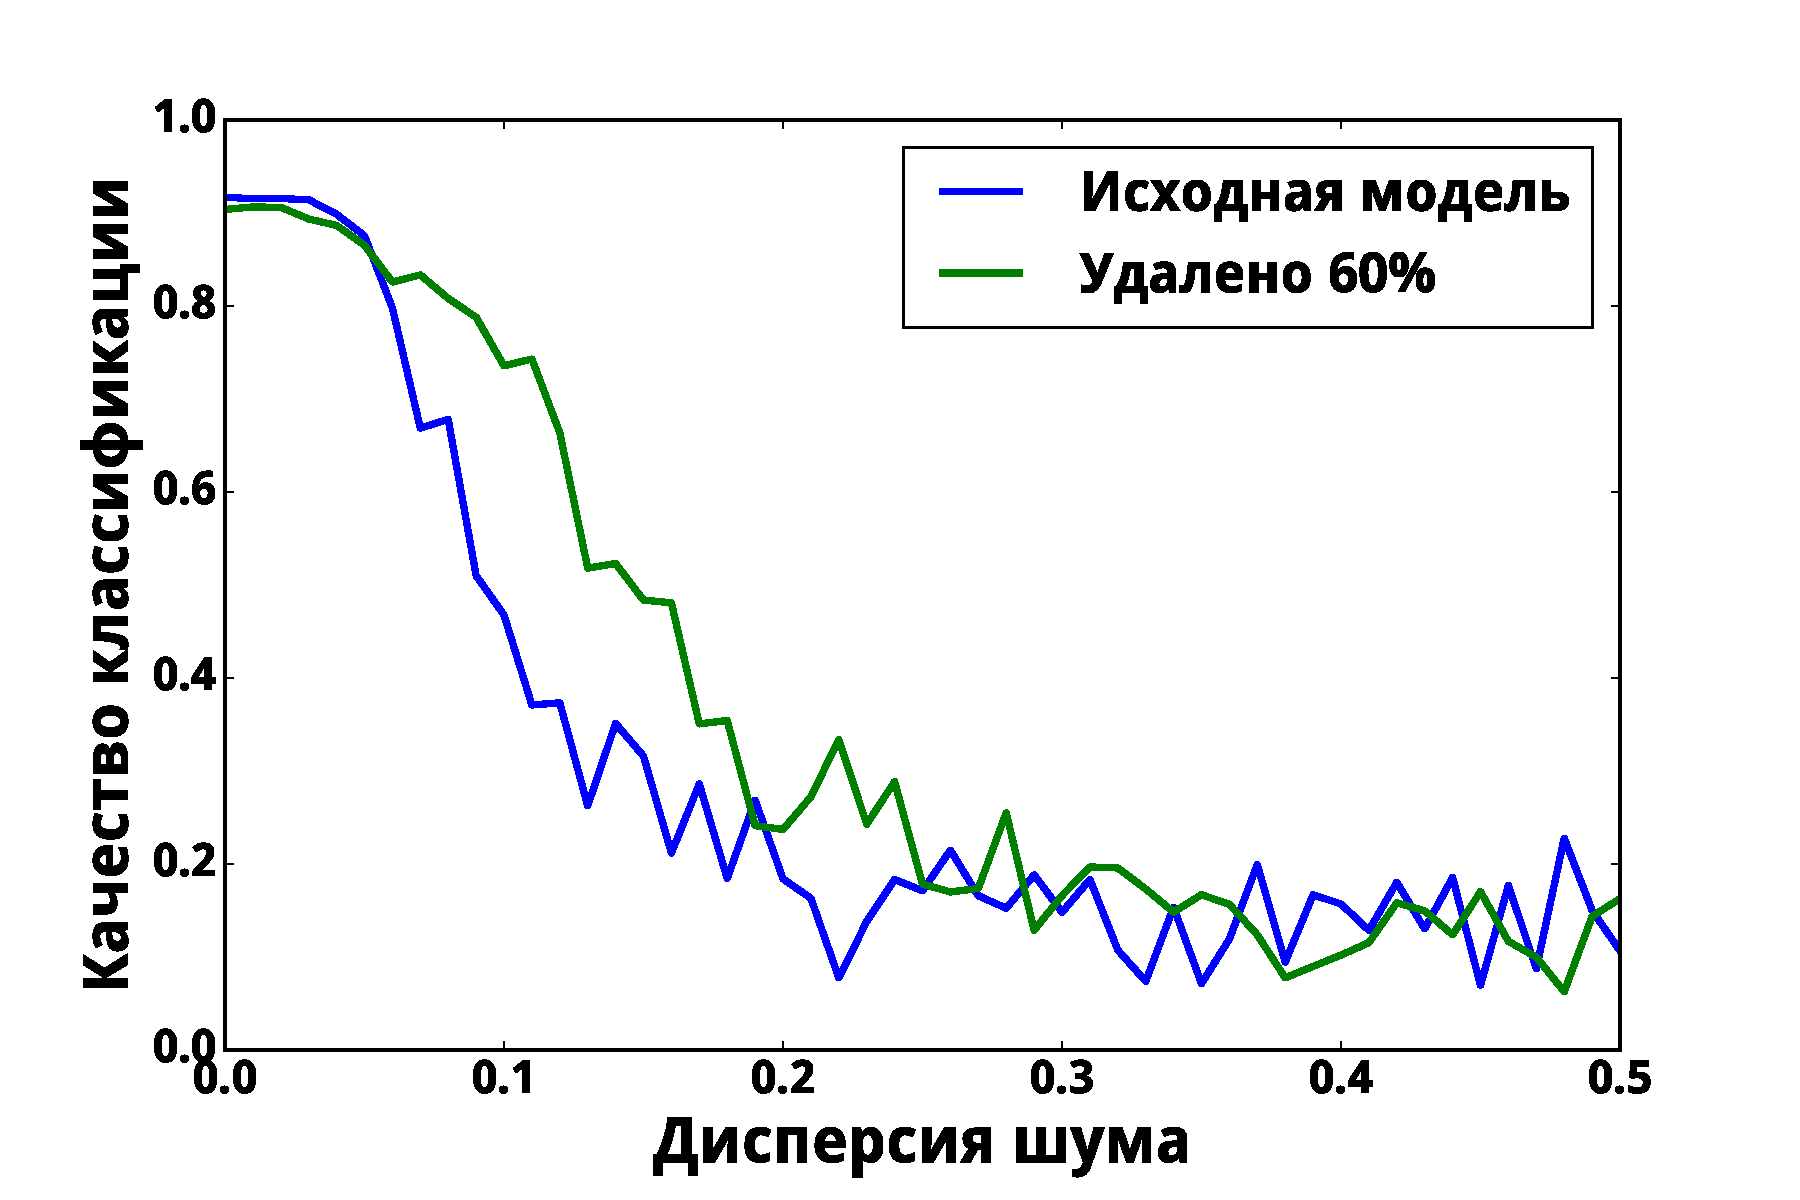
\includegraphics[width=0.55\textwidth]{./slide_plots/noise.pdf}}                                                     
\end{figure}                                                                                                   
\textcolor{gray}{Глубокое обучение предполагает оптимизацию моделей с заведомо избыточной сложностью.}  

                                                                                                                                             
\end{frame}    

\begin{frame}{Модель глубокого обучения}
\small
\begin{block}{Определение}
\textit{Моделью} $\mathbf{f}(\mathbf{w}, \mathbf{x})$ назовем непрерывно-дифференцируемую по параметрам $\mathbf{w}$ функцию из множества признаковых описаний объекта во множество меток:
\[
    \mathbf{f}: \mathbb{X} \times \mathbb{W} \to \mathbb{Y},
\] 
где $\mathbb{W}$ --- пространство параметров функции $\mathbf{f}$.
\end{block}
~\\
\textbf{Особенность задачи}  выбора модели \textit{глубокого обучения} --- значительное число параметров моделей приводит к неприменимости ряда методов оптимизации и выбора структуры модели  (AIC, BIC, кросс-валидация). \\

Модель определяется параметрами $\mathbf{w}$ и структурой $\boldsymbol{\Gamma}$.\\
\textbf{Структура} задает набор суперпозиций, входящих в модель и выбирается в согласно статистическим критериям сложности модели.\\

\textbf{Эмпирические оценки статистической сложности модели:}
\begin{enumerate}
\item число параметров;
\item число суперпозиций, из которых состоит модель.
\end{enumerate}
\end{frame}


\begin{frame}{Выбор структуры: двуслойная нейросеть}
\small
Модель $\mathbf{f}$ задана \textbf{структурой}  $\boldsymbol{\Gamma} = [\boldsymbol{\gamma}^{0,1}, {\boldsymbol{\gamma}^{1,2}}].$

\[
    \text{Модель: }\mathbf{f}(\mathbf{x}) = \textbf{softmax}\left(\mathbf{W}^{1,2}_0{\mathbf{f}_1}(\mathbf{x})\right), \quad \mathbf{f}(\mathbf{x}): \mathbb{R}^n \to [0,1]^{|\mathbb{Y}|}, \quad \mathbf{x} \in \mathbb{R}^n.
\]
\[
\mathbf{f}_1(\mathbf{x}) = {\gamma}^{0,1}_{0}\mathbf{g}^{0,1}_{0}(\mathbf{x}) + {\gamma}^{0,1}_{1}\mathbf{g}^{0,1}_{1}(\mathbf{x}),
\]
где $\mathbf{W} = [\mathbf{W}^{0,1}_0, \mathbf{W}^{0,1}_1, \mathbf{W}^{1,2}_0]^{\text{T}}$ --- матрицы параметров, $\{\mathbf{g}^{0}_{0,1},\mathbf{g}^{1}_{0,1},{\mathbf{g}^{0}_{1,2}\}}$ --- обобщенно-линейные функции скрытых слоев нейросети.

\begin{tikzpicture}[node distance=0.5cm, auto]
  %\tikzstyle{every state}=[fill=red,draw=none,text=white]

  \node (f0)  at (1,6)                  {$\mathbf{f}_0(\mathbf{x}) = \mathbf{x}$};
  %\node (g11) at (6,3)                    {$\mathbf{g}^{1,1}(\mathbf{x})$};% = \text{Conv}(\mathbf{x}, 3, 32, 1)$};
  %\node (g12)  at (6,9)                   {$\mathbf{g}^{1,2}(\mathbf{x})$};% = \text{Conv}(\mathbf{x}, 4, 32, 1)$};
  \node (f1)  at (7,6)                 {$\mathbf{f}_1(\mathbf{x})$};% = \gamma^{1,1}\mathbf{g}^{1,1}(\mathbf{x}) +  \gamma^{1,2}\mathbf{g}^{1,2}(\mathbf{x})$};
  %\node (g21) at (12,6)                   {$\mathbf{g}^{2,1}(\mathbf{x})$};% = \boldsymbol{\sigma}(\mathbf{w}^{2,1}\mathbf{x})$};
  \node (f2)  at (12,6)                   {$\mathbf{f}_2(\mathbf{x})$};% = \gamma^{2,1}\mathbf{g}^{2,1}(\mathbf{x})$};
  \path[->]  (f0) edge [bend left=50] node {$\gamma^{0,1}_0\mathbf{g}^{0,1}_0(\mathbf{x}) = \gamma^{0,1}_0\boldsymbol{\sigma}(\mathbf{W}^{0,1}_0\mathbf{x})$}(f1);
  \path[->] (f0)  edge[bend right=50] node[below] {$\gamma^{0,1}_1\mathbf{g}^{0,1}_1(\mathbf{x}) = \gamma^{0,1}_1\boldsymbol{\sigma}(\mathbf{W}^{0,1}_1\mathbf{x})$}(f1);
  \path[->] (f1)  edge node {$\gamma^{1,2}_0\mathbf{g}^{1,2}_0(\mathbf{x}) = \gamma^{1,2}_0\textbf{softmax}(\mathbf{W}^{1,2}_0\mathbf{x})$}(f2);       
  \draw[->] (f1) to (f2);
 
\end{tikzpicture}

\end{frame}


\begin{frame}{Графовое представление модели глубокого обучения}
\footnotesize
Заданы:
\begin{enumerate}
 \item ациклический граф $(V,E)$;
\item для каждого ребра $(j,k) \in E$: вектор базовых липшецевых функций  $\mathbf{g}^{j,k} = [\mathbf{g}^{j,k}_0, \dots, \mathbf{g}^{j,k}_{K^{j,k}}]$  мощности $K^{j,k}$;
\item для каждой вершины $v \in V$: липшецевая функция агрегации $\textbf{agg}_v$.
\item Функция $\mathbf{f} = \mathbf{f}_{|V|-1}$, задаваемая по правилу 
\begin{equation}
\label{eq:modelfam}
    \mathbf{f}_{v}(\mathbf{w}, \mathbf{x}) = \textbf{agg}_{v}\left(\{ \langle \boldsymbol{\gamma}^{j,k}, \mathbf{g}^{j,k} \rangle \circ  \mathbf{f}_j(\mathbf{x})| j \in \text{Adj}(v_k)\}\right), v \in \{1,\dots,|V|-1\}, \quad \mathbf{f}_0(\mathbf{x}) = \mathbf{x}
\end{equation}
и являющаяся функцией из признакового пространства $\mathbb{X}$ в пространство меток $\mathbb{Y}$ при значениях векторов, $\boldsymbol{\gamma}^{j,k} \in [0,1]^{K^{j,k}}$.
\end{enumerate}

\begin{block}{Определение}
Граф $(V, E)$ со множестом векторов базовых функций $\{\mathbf{g}^{j,k}, (j,k) \in E\}$ и функций агрегаций $\{ \textbf{agg}_v, {v \in V}\}$ назовем \textit{параметрическим семейством моделей} $\mathfrak{F}$.
\end{block}
\begin{block}{Утверждение}
Для любого значения $\boldsymbol{\gamma}^{j,k} \in [0,1]^{K^{j,k}}$ функция $\mathbf{f} \in \mathfrak{F}$ является моделью.
\end{block}
\end{frame}

      

\begin{frame}{Ограничения на структурные параметры}
Примеры ограничений для одного структурного параметра $\boldsymbol{\gamma}, |\boldsymbol{\gamma}| = 3$.
\begin{figure}
 \begin{minipage}[t]{.45\textwidth}
        \centering
%1 limit
\begin{tikzpicture}[%
x={(1.5cm,0cm)},
y={(0cm,1.5cm)},
z={({0.5*cos(45)},{0.5*sin(45)})},
]

\coordinate (A) at (0,0,0); 
\coordinate (B) at (1,0,0) ;
\coordinate (C) at (1,1,0); 
\coordinate (D) at (0,1,0); 
\coordinate (E) at (0,0,1); 
\coordinate (F) at (1,0,1); 
\coordinate (G) at (1,1,1); 
\coordinate (H) at (0,1,1   );

%Ecken
\node[circle,scale=0.5,fill=black,draw=black](Ap) at (0,0,0){};
\node[circle,scale=0.5,fill=black,draw=black](Bp) at (1,0,0){};
\node[circle,scale=0.5,fill=black,draw=black](Cp) at (1,1,0){};
\node[circle,scale=0.5,fill=black,draw=black](Dp) at (0,1,0){};
\node[circle,scale=0.5,fill=black,draw=black](Ep) at (0,0,1){};
\node[circle,scale=0.5,fill=black,draw=black](Fp) at (1,0,1){};
\node[circle,scale=0.5,fill=black,draw=black](Gp) at (1,1,1){};
\node[circle,scale=0.5,fill=black,draw=black](Hp) at (0,1,1){};
\node[left= 1pt of A]{[0,0,0]};
\node[right= 1pt of B]{[1,0,0]};
\node[right= 1pt of C]{[1,1,0]};
\node[left= 1pt of D]{[0,1,0]};
\node[left= 1pt of E]{[0,0,1]};
\node[right= 1pt of F]{[1,0,1]};
\node[right= 1pt of G]{[1,1,1]};
\node[left= 1pt of H]{[0,1,1]};

%Kanten
\draw[] (A)
-- (B)  node[midway, below]{}
-- (C)      node[midway, right]{}
-- (D)  node[midway, above]{}
-- (A)  node[midway, left]{};
\draw[] (B) -- (F) -- (G) -- (C);
\draw[] (G) -- (H) -- (D);
\draw[densely dashed] (A) -- (E) -- (F);
\draw[densely dashed] (E) -- (H);

\end{tikzpicture}
\caption*{На вершинах куба}
\end{minipage}
\hfill
 \begin{minipage}[t]{.45\textwidth}
        \centering

%2 limit
\begin{tikzpicture}[%
x={(1.5cm,0cm)},
y={(0cm,1.5cm)},
z={({0.5*cos(45)},{0.5*sin(45)})},
]

\coordinate (A) at (0,0,0); 
\coordinate (B) at (1,0,0) ;
\coordinate (C) at (1,1,0); 
\coordinate (D) at (0,1,0); 
\coordinate (E) at (0,0,1); 
\coordinate (F) at (1,0,1); 
\coordinate (G) at (1,1,1); 
\coordinate (H) at (0,1,1   );

%Ecken
\node[left= 1pt of A]{[0,0,0]};
\node[right= 1pt of B]{[1,0,0]};
\node[right= 1pt of C]{};
\node[left= 1pt of D]{[0,1,0]};
\node[left= 1pt of E]{};
\node[right= 1pt of F]{[1,0,1]};
\node[right= 1pt of G]{[1,1,1]};
\node[left= 1pt of H]{[0,1,1]};

%Kanten
\draw[fill=gray] (A)
-- (B)  node[midway, below]{}
-- (C)      node[midway, right]{}
-- (D)  node[midway, above]{}
-- (A)  node[midway, left]{};
\draw[fill=gray] (B) -- (F) -- (G) -- (C);
\draw[fill=gray] (G) -- (H) -- (D);
\draw[fill=gray] (A) -- (E) -- (F);
\draw[fill=gray] (E) -- (H);
\draw[fill=gray] (D) -- (H) -- (G) -- (C);
\end{tikzpicture}
\caption*{Внутри куба}
\end{minipage}
\hfill
 \begin{minipage}[t]{.45\textwidth}
        \centering
%3 limit
\begin{tikzpicture}[%
x={(1.5cm,0cm)},
y={(0cm,1.5cm)},
z={({0.5*cos(45)},{0.5*sin(45)})},
]

\coordinate (A) at (0,0,0); 
\coordinate (B) at (1,0,0) ;
\coordinate (C) at (1,1,0); 
\coordinate (D) at (0,1,0); 
\coordinate (E) at (0,0,1); 
\coordinate (F) at (1,0,1); 
\coordinate (G) at (1,1,1); 
\coordinate (H) at (0,1,1   );

%Ecken
\node[circle,scale=0.5,fill=black,draw=black](Bp) at (1,0,0){};
\node[circle,scale=0.5,fill=black,draw=black](Dp) at (0,1,0){};
\node[circle,scale=0.5,fill=black,draw=black](Ep) at (0,0,1){};
\node[left= 1pt of A]{};
\node[right= 1pt of B]{[1,0,0]};
\node[right= 1pt of C]{};
\node[left= 1pt of D]{[0,1,0]};
\node[left= 1pt of E]{[0,0,1]};
\node[right= 1pt of F]{};
\node[right= 1pt of G]{};
\node[left= 1pt of H]{};

%Kanten
\draw[] (A)
-- (B)  node[midway, below]{}
-- (C)      node[midway, right]{}
-- (D)  node[midway, above]{}
-- (A)  node[midway, left]{};
\draw[] (B) -- (F) -- (G) -- (C);
\draw[] (G) -- (H) -- (D);
\draw[densely dashed] (A) -- (E) -- (F);
\draw[densely dashed] (E) -- (H);

\end{tikzpicture}
\caption*{На вершинах симплекса}
\end{minipage}
\hfill
 \begin{minipage}[t]{.45\textwidth}
        \centering
%4 limit
\begin{tikzpicture}[%
x={(1.5cm,0cm)},
y={(0cm,1.5cm)},
z={({0.5*cos(45)},{0.5*sin(45)})},
]

\coordinate (A) at (0,0,0); 
\coordinate (B) at (1,0,0) ;
\coordinate (C) at (1,1,0); 
\coordinate (D) at (0,1,0); 
\coordinate (E) at (0,0,1); 
\coordinate (F) at (1,0,1); 
\coordinate (G) at (1,1,1); 
\coordinate (H) at (0,1,1   );

%Ecken
\node[left= 1pt of A]{};
\node[right= 1pt of B]{[1,0,0]};
\node[right= 1pt of C]{};
\node[left= 1pt of D]{[0,1,0]};
\node[left= 1pt of E]{[0,0,1]};
\node[right= 1pt of F]{};
\node[right= 1pt of G]{};
\node[left= 1pt of H]{};

%Kanten
\draw[] (A)
-- (B)  node[midway, below]{}
-- (C)      node[midway, right]{}
-- (D)  node[midway, above]{}
-- (A)  node[midway, left]{};
\draw[] (B) -- (F) -- (G) -- (C);
\draw[] (G) -- (H) -- (D);
\draw[densely dashed] (A) -- (E) -- (F);
\draw[densely dashed] (E) -- (H);
\draw[fill=gray] (B) -- (D) -- (E);


\end{tikzpicture}
\caption*{Внутри симплекса}
\end{minipage}

\end{figure}

\end{frame}






\begin{frame}{Априорное распределение параметров}
\footnotesize   
\begin{columns}
\begin{column}{0.6\textwidth}
   \begin{block}{Определение}
\textit{Априорным распределением} параметров $\mathbf{W}$ и структуры  $\boldsymbol{\Gamma}$ модели $\mathbf{f}$ назовем вероятностное распределение
$
    p(\mathbf{W}, \boldsymbol{\Gamma}|\mathbf{h}): \mathbb{W} \times \amsmathbb{\Gamma} \times \mathbb{H} \to \mathbb{R}^{+}, 
$
где $\mathbb{W}$ --- множество значений параметров модели, $\amsmathbb{\Gamma}$~---~множество значений структуры модели.
\end{block}

\end{column}
\begin{column}{0.4\textwidth}  %%<--- here
    \begin{center}
     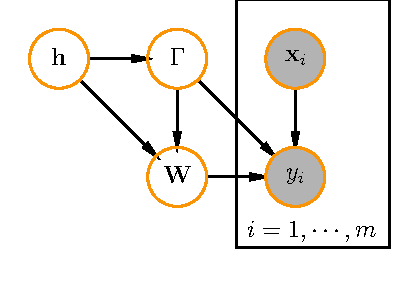
\includegraphics[width=\textwidth]{simple_plate.pdf}
     \end{center}
\end{column}
\end{columns}
\vspace*{-0.5cm}
\begin{block}{Определение}
\textit{Гиперпараметрами} $\mathbf{h}\in \mathbb{H}$ модели  назовем параметры распределения $p(\mathbf{w}, \boldsymbol{\Gamma}|\mathbf{h})$ (параметры распределения параметров модели $\mathbf{f}$).
 
\end{block}
Модель $\mathbf{f}$ задается следующими величинами:
\begin{itemize}
\item \textbf{Параметры} $\mathbf{W} \in \mathbb{W}$ задают суперпозиции $\mathbf{f}_v$, из которых состоит модель $\mathbf{f}$.
\item \textbf{Структурные параметры} $\boldsymbol{\Gamma} \in \amsmathbb{\Gamma}$ задают вклад суперпозиций $\mathbf{f}_v$ в модель $\mathbf{f}$.
\item \textbf{Гиперпараметры} $\mathbf{h} \in \mathbb{H}$ задают распределение параметров и структурных параметров модели.
\item \textbf{Метапараметры} $\boldsymbol{\beta} \in \mathbb{B}$ задают вид оптимизации модели.
\end{itemize}

\end{frame}






\begin{frame}{Априорное распределение на структуре модели}
Каждая точка на симплексе задает модель.

\textbf{Распределение Дирихле: }$\boldsymbol{\Gamma}\sim \text{Dir}(\mathbf{s}, c_\text{temp})$\\
\begin{figure}
 \begin{minipage}[t]{.3\textwidth}
        \centering
\begin{tikzpicture}[%
x={(1.7cm,0cm)},
y={(0cm,1.7cm)},
]

\coordinate (A) at (0,0); 
\coordinate (B) at (1,0) ;
\coordinate (C) at (0.5,0.86); 

%Ecken
\node[circle,scale=0.5,fill=black,draw=black](Ap) at (0,0){};
\node[circle,scale=0.5,fill=black,draw=black](Bp) at (1,0){};
\node[circle,scale=0.5,fill=black,draw=black](Cp) at (0.5,0.86){};

%Kanten
\draw[] (A)
-- (B)  node[midway, below]{}
-- (C)      node[midway, right]{}
-- (A)  node[midway, left]{};

\end{tikzpicture}
\caption*{$c_\text{temp}\to0$}
\end{minipage}
\hfill
 \begin{minipage}[t]{.3\textwidth}
   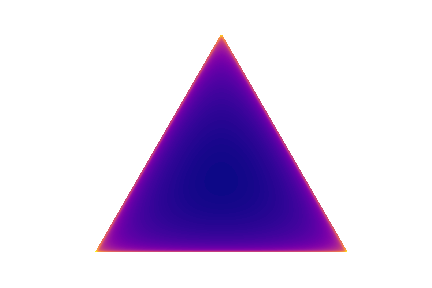
\includegraphics[width=\textwidth]{dir0995.png}
\caption*{$c_\text{temp}=0.995$}
\end{minipage}
\hfill
 \begin{minipage}[t]{.3\textwidth}
   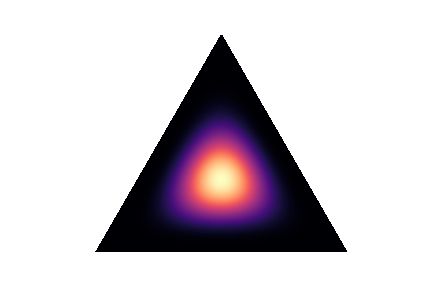
\includegraphics[width=\textwidth]{dir5.png}
\caption*{$c_\text{temp}=5.0$}
\end{minipage}

\end{figure}

\textbf{Распределение Гумбель-софтмакс: }$\boldsymbol{\Gamma}\sim \text{GS}(\mathbf{s}, c_\text{temp})$\\
\begin{figure}
 \begin{minipage}[t]{.3\textwidth}
        \centering
\begin{tikzpicture}[%
x={(1.7cm,0cm)},
y={(0cm,1.7cm)},
]

\coordinate (A) at (0,0); 
\coordinate (B) at (1,0) ;
\coordinate (C) at (0.5,0.86); 

%Ecken
\node[circle,scale=0.5,fill=black,draw=black](Ap) at (0,0){};
\node[circle,scale=0.5,fill=black,draw=black](Bp) at (1,0){};
\node[circle,scale=0.5,fill=black,draw=black](Cp) at (0.5,0.86){};

%Kanten
\draw[] (A)
-- (B)  node[midway, below]{}
-- (C)      node[midway, right]{}
-- (A)  node[midway, left]{};

\end{tikzpicture}
\caption*{$c_\text{temp}\to0$}
\end{minipage}
\hfill
 \begin{minipage}[t]{.3\textwidth}
   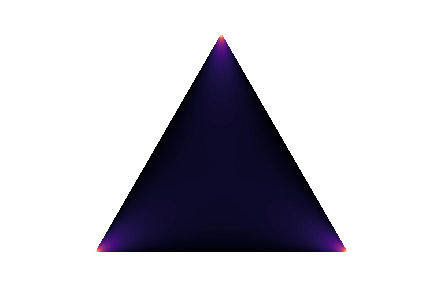
\includegraphics[width=\textwidth]{gs0995.png}
\caption*{$c_\text{temp}=0.995$}
\end{minipage}
\hfill
 \begin{minipage}[t]{.3\textwidth}
   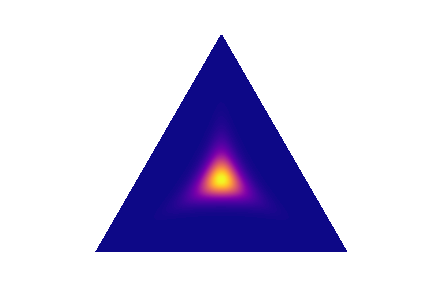
\includegraphics[width=\textwidth]{gs5.png}
\caption*{$c_\text{temp}=5.0$}
\end{minipage}

\end{figure}
\end{frame}


\begin{frame}{Байесовский выбор модели}


\begin{columns}
\begin{column}{0.4\textwidth}
Базовая модель %https://www.microsoft.com/en-us/research/wp-content/uploads/2016/02/bishop-variational-icann-98.pdf
\begin{itemize}
\item \textbf{Параметры} модели:\\ $\mathbf{W} \sim \mathcal{N}(0, \alpha^{-1}),$
\item \textbf{Гиперпараметры} модели: $\mathbf{h} = [\alpha].$
\end{itemize}
\begin{figure}
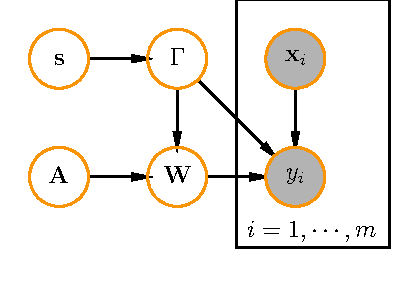
\includegraphics[width=\textwidth]{simple_plate_concrete.pdf}
\end{figure}
\end{column}
\begin{column}{0.6\textwidth}
\textbf{Предлагаемая модель  }
\begin{itemize}
\item \textbf{Параметры} модели:\\ $\mathbf{W}_r^{j,k} \sim \mathcal{N}(0, \gamma_{r}^{j,k} (\mathbf{A}_r^{j,k})^{-1}),$
$\mathbf{A}_r^{j,k}$ --- диагональная матрица параметров, соответствующих подмодели $\mathbf{g}_r^{j,k}$,
\\$\mathbf{A}_r^{j,k} \sim \text{inv-gamma}(c_1,c_2)$.

\item \textbf{Структурные параметры} модели:\\$\boldsymbol{\Gamma} = \{\boldsymbol{\gamma}^{j,k}, (j,k) \in E\},$ \\$\boldsymbol{\gamma}^{j,k} \sim \text{GS}(\mathbf{s}^{j,k}, c_\text{temp}).$ 
\item \textbf{Гиперпараметры} модели: $\mathbf{h} = \{\mathbf{A}, \mathbf{s} \}.$
\item \textbf{Метапараметры:} $c_1,c_2,c_\text{temp}$.
\end{itemize}

\end{column}

\end{columns}

%

\end{frame}


\begin{frame}{Правдоподобие как статистическая сложность}  
\footnotesize
\textbf{Статистическая сложность} модели $\mathbf{f}$:
\[
	\text{MDL}(\mathbf{y},\mathbf{f}) = \textcolor{OliveGreen}{-\text{log}~p(\mathbf{h})} - \text{log}~\bigl(p(\mathbf{y}|\mathbf{X}, \mathbf{h})\delta\mathfrak{D})\bigr),
\]
где $\delta\mathfrak{D}$ --- допустимая точность передачи информации о выборке $\mathfrak{D}$.\\~\\

Выбор значений гиперпараметров производится в согласно \textbf{правдоподобию модели} $Q$:                                      
\[                                                                                                                                              
        Q(\mathbf{h}|  \boldsymbol{\theta}^{*}, \mathbf{X}, \mathbf{y} ) = \text{log}p(\mathbf{h}|\mathbf{X}, \mathbf{y})= \textcolor{OliveGreen}{\text{log}p(\mathbf{h})} +  \text{log}\iint\limits_{\mathbf{W}, \boldsymbol{\Gamma}} \textcolor{red}{p(\mathbf{y}|\mathbf{X},\mathbf{W},  \boldsymbol{\Gamma})} \textcolor{blue}{p(\mathbf{W}, \boldsymbol{\Gamma}| \mathbf{h})} d\mathbf{W}d{\boldsymbol{\Gamma}},                         
\]       
Выбор значений параметров $\mathbf{W}$ производится  согласно \textbf{апостериорному распределению параметров} $L$:                                      
\[
     L(\boldsymbol{\theta}|  \mathbf{h},  \mathbf{X}, \mathbf{y}) =   \text{log} p(\mathbf{W}, \boldsymbol{\Gamma}|\mathbf{X}, \mathbf{y}, \mathbf{h}) \propto  \textcolor{red}{\text{log} p(\mathbf{y}|\mathbf{X},\mathbf{W},\boldsymbol{\Gamma}, \mathbf{h})} +  \textcolor{blue}{\text{log} p(\mathbf{W}, \boldsymbol{\Gamma}|\mathbf{h})}.
\]

\begin{figure}
\vspace{-0.5cm}
  \centering
 \subfloat[Выбор модели по правдоподобию]{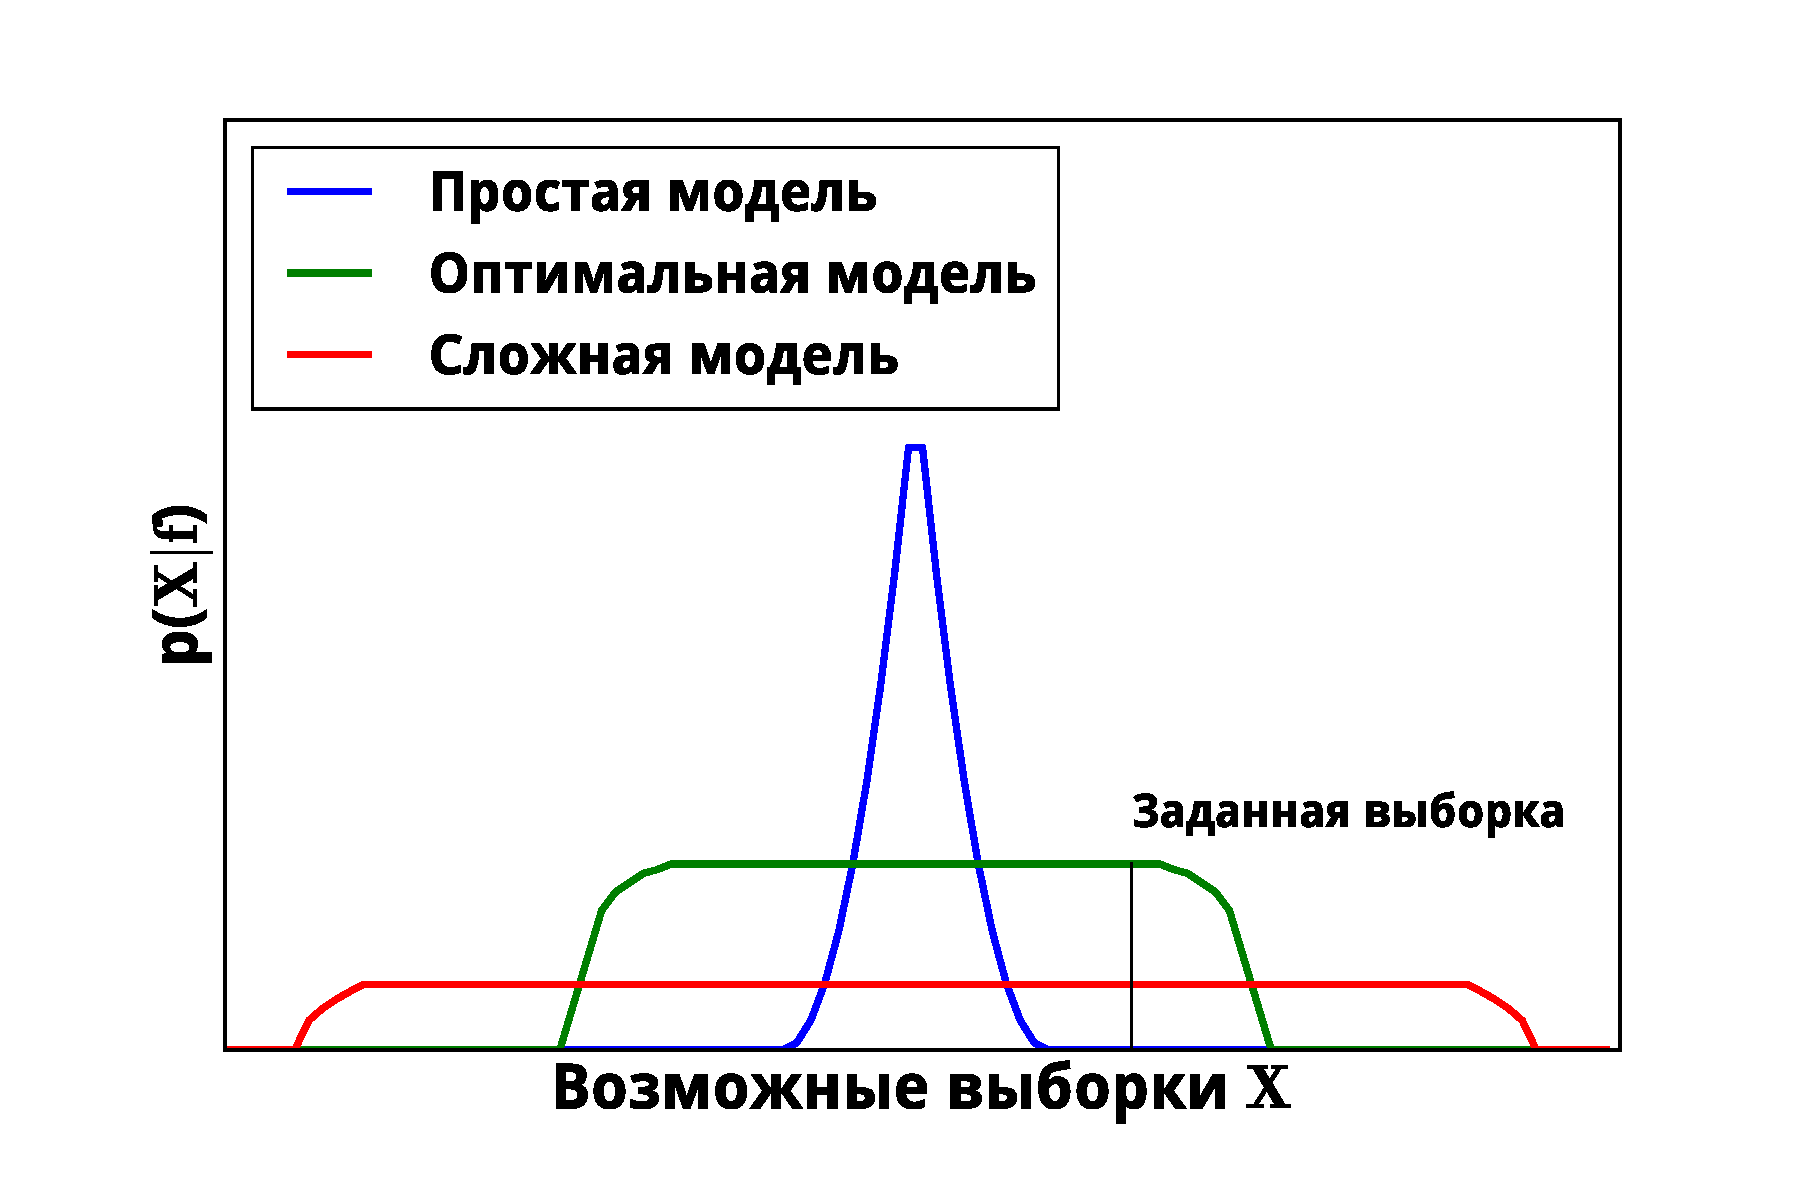
\includegraphics[width=0.45\textwidth]{slide_plots/evidence.pdf}} 
 \subfloat[Аппроксимация выборки полиномами]{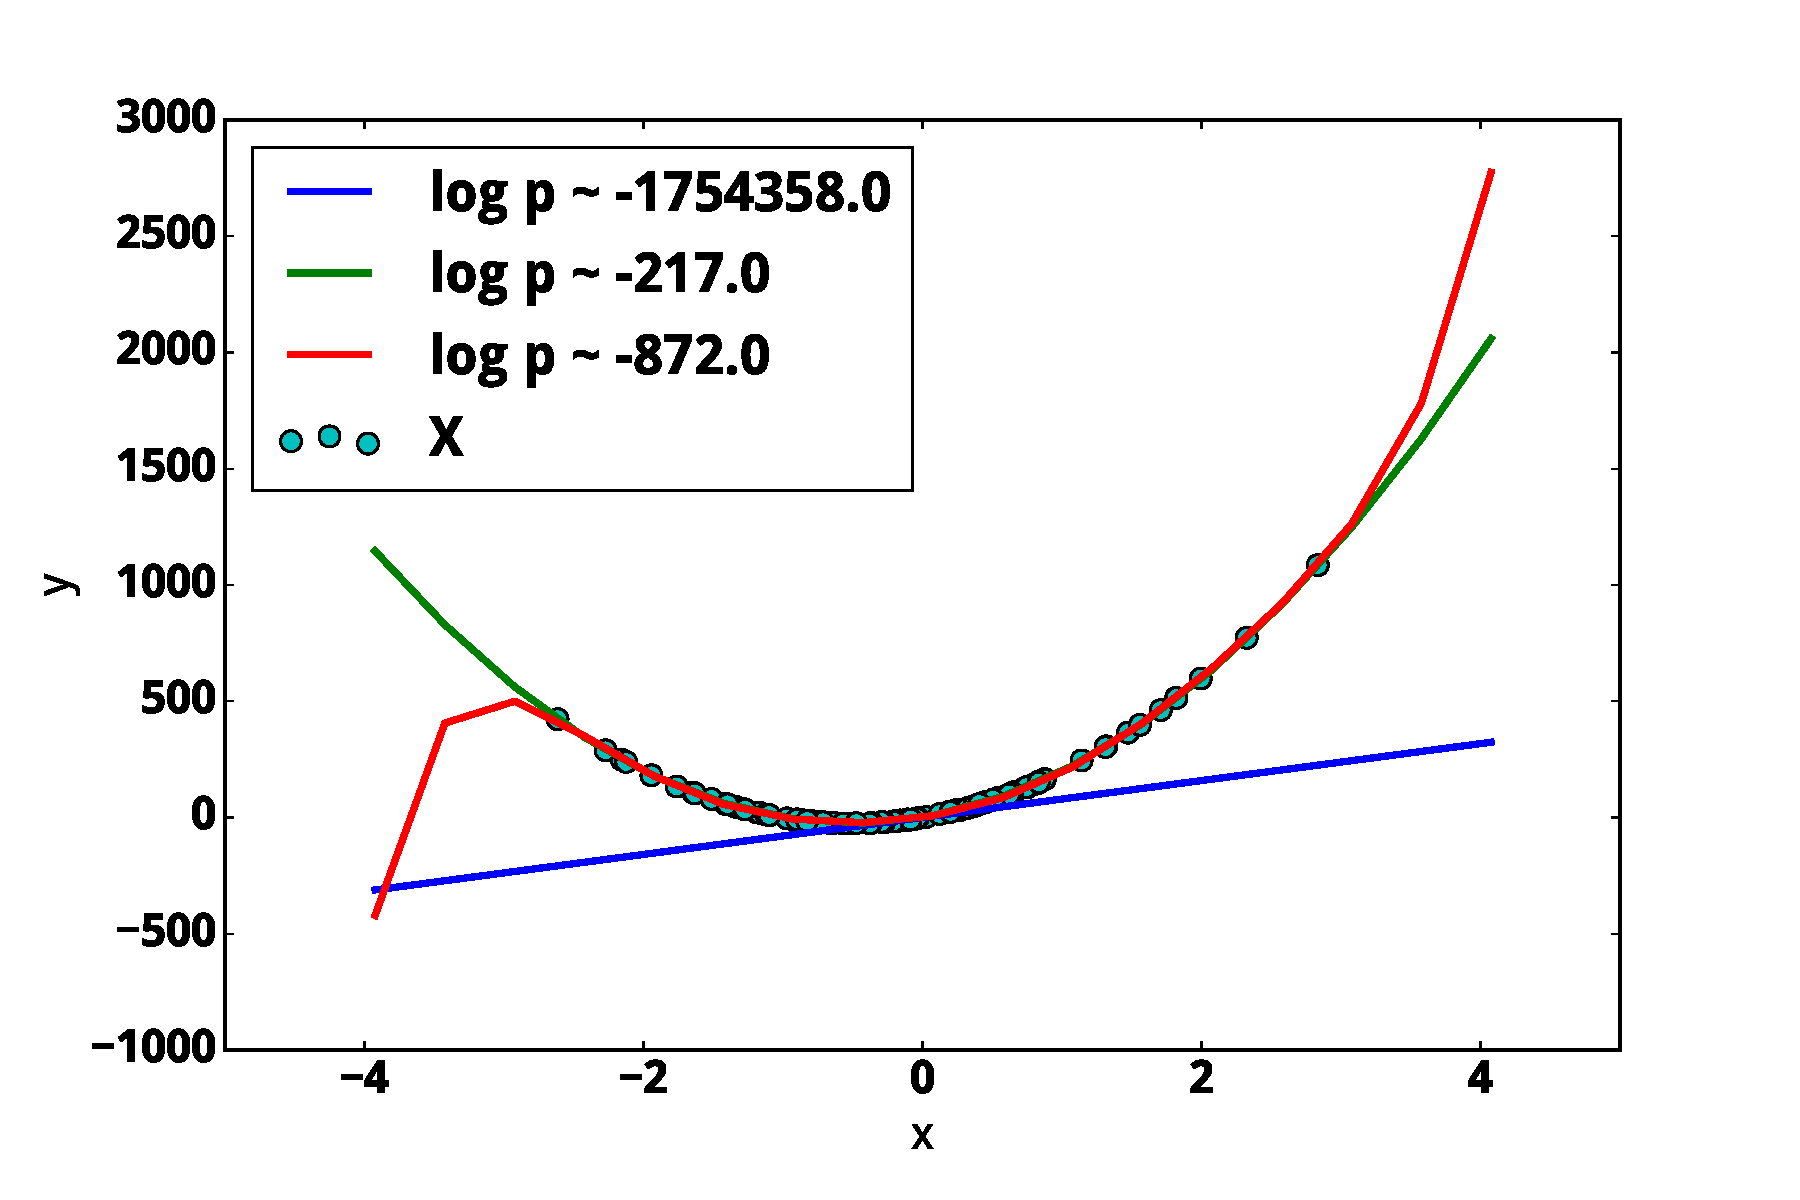
\includegraphics[width=0.45\textwidth]{slide_plots/example.pdf}}

\end{figure}
\end{frame}


\begin{frame}{Вариационная нижняя оценка правдоподобия} 
\footnotesize

Интеграл правдоподобия невычислим аналитически.\\
\textbf{Правдоподобие модели:}
\[
p(\mathbf{y}|\mathbf{X}, c_\text{temp}) =
 \iint\limits_{\mathbf{W}, \boldsymbol{\Gamma}}  \textcolor{red}{p(\mathbf{y}|\mathbf{X},\mathbf{W},  \boldsymbol{\Gamma})} \textcolor{blue}{p(\mathbf{W}, \boldsymbol{\Gamma}| c_\text{temp})}d\mathbf{W}d{\boldsymbol{\Gamma}}.                         
\]

\begin{columns}
\begin{column}{0.55\textwidth}
  
\begin{block}{Определение}
\textit{Вариационными параметрами} модели $\boldsymbol{\theta} \in \mathbb{R}^{{u}}$ назовем параметры распределения $q$, приближающие апостериорное распределение параметров и структур $p(\mathbf{W}, \boldsymbol{\Gamma}|\mathbf{X}, \mathbf{y}, \mathbf{h}, c_\text{temp})$:
\[
    q \approx  \frac{p(\mathbf{y}|\mathbf{X},\mathbf{W},\boldsymbol{\Gamma})p(\mathbf{W}, \boldsymbol{\Gamma}|\mathbf{h}, c_\text{temp})}{\iint\limits_{\mathbf{W}', \boldsymbol{\Gamma'}}p(\mathbf{y}|\mathbf{X},\mathbf{W}',\boldsymbol{\Gamma}')p(\mathbf{W}', \boldsymbol{\Gamma}'|\mathbf{h}, c_\text{temp})d\mathbf{W}'d\boldsymbol{\Gamma}'}.
\]
\end{block} 

\end{column}
\begin{column}{0.45\textwidth}  %%<--- here
    \begin{center}
     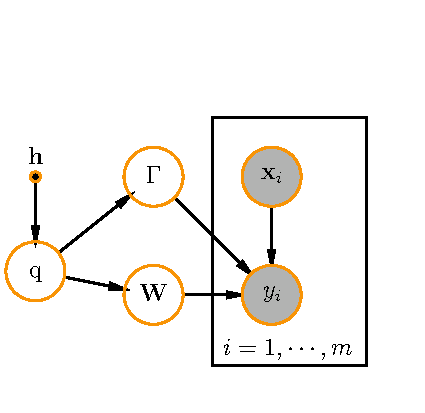
\includegraphics[width=\textwidth]{plate.pdf}
     \end{center}
\end{column}
\end{columns}



%Пусть $q(\mathbf{W}, \boldsymbol{\Gamma}) = q_{\mathbf{W}}(\mathbf{W})q_{\boldsymbol{\Gamma}}(\boldsymbol{\Gamma})$ --- непрерывное распределение, аппроксимирующее 
%апостериорное распределение $p(\mathbf{W}, \boldsymbol{\Gamma}|\mathbf{y}, \mathbf{X})$.
~\\Получим нижнюю оценку интеграла правдоподобия.
$$                                                                                                                                              
        \text{log}~p(\mathbf{y}|\mathbf{X}, c_\text{temp}) \geq 
\textcolor{blue}{\mathsf{E}_q \text{log}~{p(\mathbf{y} | \mathbf{X}, \mathbf{W}, \boldsymbol{\Gamma})}} - \textcolor{red}{\text{D}_{KL}(q(\mathbf{W}, \boldsymbol{\Gamma})||p(\mathbf{w}, \boldsymbol{\Gamma}, c_\text{temp}))} = \text{log}\hat{{p}}(\mathbf{y}|\mathbf{X}, c_\text{temp}).
$$ 



Оценка совпадает с интегралом правдоподобия при $$D_\text{KL}(q(\mathbf{W}, \boldsymbol{\Gamma})|(p(\mathbf{W}, \boldsymbol{\Gamma}|\mathbf{y}, \mathbf{X}, c_\text{temp}))=0.$$

\end{frame}      


\begin{frame}{Задача выбора модели}
\footnotesize
Зададим вариационное распределение $q$ с параметрами $\boldsymbol{\theta}$, приближающие апостериорное распределение $p(\mathbf{W}, \boldsymbol{\Gamma}|\mathbf{X}, \mathbf{y}, \mathbf{h})$ параметров и структуры.



\begin{block}{Определение}

\textit{Функцией потерь} $L( \boldsymbol{\theta}| \mathbf{h}, \mathbf{X}, \mathbf{y})$   назовем дифференцируемую функцию, качество модели на обучающей выборки при параметрах $\boldsymbol{\theta}$ распределения $q$.
\end{block}
\begin{block}{}
\textit{Функцией валидации} $Q(\mathbf{h}| \boldsymbol{\theta}, \mathbf{X}, \mathbf{y} )$ назовем дифференцируемую функцию, качество модели при векторе $\boldsymbol{\theta}$, заданном неявно.
\end{block}
\begin{block}{}
\textit{Задачей выбора модели} $\mathbf{f}$ назовем двухуровневую задачу оптимизации:

\[
	\mathbf{h}^{*} = \argmin_{\mathbf{h} \in \mathbb{H}} Q(\mathbf{h}|  \boldsymbol{\theta}^{*}, \mathbf{X}, \mathbf{y} ),
\]
где $\boldsymbol{\theta}^{*}$ --- решение задачи оптимизации
\[
   \boldsymbol{\theta}^{*} = \argmin_{\boldsymbol{\theta} \in \mathbb{R}^u} L(\boldsymbol{\theta}|  \mathbf{h},  \mathbf{X}, \mathbf{y}).
\]
\end{block}


\end{frame}







                                                                                                              


   
\begin{frame}{Общая задача}
\tiny
\begin{block}{Определение}
Задачу выбора модели $\mathbf{h}^{*}, \boldsymbol{\theta}^{*}$ назовем обобщаюшей, если выполнены следующие условия:
\begin{enumerate}
\item \textit{Условие оптимизации максимума правдоподобия выборки:} существует значение гиперпараметров $\boldsymbol{\beta}$ и константа $K$, такие что для любых векторов гиперпараметров $\mathbf{h}_1, \mathbf{h}_2, Q(\mathbf{h}_1) - Q(\mathbf{h}_2) > K:$ соответствующие матожидания правдоподбия выборок упорядочены как $\mathsf{E}_q \text{log}~p(\mathbf{y}|\boldsymbol{\theta}_1, c_{\text{temp}})>\text{log}\mathsf{E}_q ~p(\mathbf{y}|\boldsymbol{\theta}_2, c_{\text{temp}})$

\item \textit{Условие минимизации сложности модели:} существует значение гиперпараметров $\boldsymbol{\beta}$ и константа $K$, такие что для любых векторов гиперпараметров $\mathbf{h}_1, \mathbf{h}_2, Q(\mathbf{h}_1) - Q(\mathbf{h}_2) > K$ и таких что  соответствующие матожидания правдоподбия выборок равны: $\mathsf{E}_q \text{log}~p(\mathbf{y}|\boldsymbol{\theta}_1, c_{\text{temp}}) = \text{log}\mathsf{E}_q ~p(\mathbf{y}|\boldsymbol{\theta}_2, c_{\text{temp}})$, количество ненулевых параметров у первой модели меньше, чем у второй.

\item \textit{Условие достижения максимума правдоподобия модели:} существует значение гиперпараметров $\boldsymbol{\beta}$, такое что оптимизация задачи эквивалента оптимизации правдоподобия модели:
\[
    \mathbf{h}^{*} = \argmax_{h'} p(\mathbf{y}|\mathbf{X}, \mathbf{h}', c_{\text{temp}}),
\]
\[
    q(\boldsymbol{\theta}^{*}) = p(\mathbf{w}, \boldsymbol{\Gamma}|\mathbf{y}, \mathbf{X}, c_{\text{temp}}).
\]

\item \textit{Условие многоэкстремальености:}
 для любых двух векторов $\mathbf{h}_{1}, \mathbf{h}_2$ и соответствующих векторов $\boldsymbol{\theta}_1^{*},\boldsymbol{\theta}_2^{*}$ существуют значения гиперпараметров $\exists \boldsymbol{\beta_1},\boldsymbol{\beta_2}$, такие что  $Q(\mathbf{h}_1, \beta_1) > Q(\mathbf{h}_2, \beta_1), Q(\mathbf{h}_1, \beta_1) < Q(\mathbf{h}_2, \beta_2)$.

\item Условие непрерывности: $\mathbf{h}^{*}, \boldsymbol{\theta}^{*}$ непрерывны по гиперпараметрам.

\end{enumerate}
\end{block}
\end{frame}
\begin{frame}{Анализ задач выбора моделей}
\begin{block}{Теорема}
Следующие задачи выбора модели не являются обобщающими:
\begin{enumerate}
\item метод максимума правдоподобия: $\textcolor{blue}{\mathsf{E}_q \text{log} p(\mathbf{y}|\mathbf{X}, \boldsymbol{\theta}, c_\text{temp})} \to \max_{\boldsymbol{\theta}};$
\item метод максимума апостериорной вероятности $\textcolor{blue}{\mathsf{E}_q \text{log} p(\mathbf{y}|\mathbf{X},  \boldsymbol{\theta})}\textcolor{red}{p( \boldsymbol{\theta}| \mathbf{h}, c_\text{temp})} \to \max_{\boldsymbol{\theta}};$
\item метод максимума вариационной оценки правдоподобия модели $\max_{\boldsymbol{\theta}} \textcolor{blue}{\mathsf{E}_q \text{log}~{p(\mathbf{y} | \mathbf{X}, \mathbf{W}, \boldsymbol{\Gamma})}} - \textcolor{red}{\text{D}_{KL}(q(\mathbf{W}, \boldsymbol{\Gamma})||p(\mathbf{w}, \boldsymbol{\Gamma}, c_\text{temp}))} \to \max_{\mathbf{h}};$
\item кросс-валидация $\textcolor{blue}{\mathsf{E}_q \text{log}p(\mathbf{y}_\text{valid}|\mathbf{X}_\text{valid}, \boldsymbol{\theta}^{*})} \to \max_{\mathbf{h}}$, $\boldsymbol{\theta}^{*} = \argmax_{\boldsymbol{\theta}} \textcolor{blue}{\mathsf{E}_q \text{log}p(\mathbf{y}_\text{train}|\mathbf{X}_\text{train}, \boldsymbol{\theta})}\textcolor{red}{p(\boldsymbol{\theta}| \mathbf{h})}$.
\item AIC: $\textcolor{blue}{\mathsf{E}_q \text{log} p(\mathbf{y}|\mathbf{X}, \boldsymbol{\theta}, c_\text{temp})} + \textcolor{red}{|\theta_i: \theta_i \neq 0|} \to \max$;
\item BIC: $\textcolor{blue}{\mathsf{E}_q \text{log} p(\mathbf{y}|\mathbf{X}, \boldsymbol{\theta}, c_\text{temp})} + \textcolor{red}{\text{log}(m)|\theta_i: \theta_i \neq 0|} \to \max$;
\item перебор структуры модели:  $\max_{\boldsymbol{\theta}} \textcolor{blue}{\mathsf{E}_q \text{log} p(\mathbf{y}|\mathbf{X}, \boldsymbol{\theta}, c_\text{temp})}\textcolor{red}{\mathbb{I}(\boldsymbol{\Gamma} = \boldsymbol{\Gamma}') }\to \max{\boldsymbol{\Gamma}'}.$
\end{enumerate}
\end{block}
\end{frame}

\begin{frame}{Общая задача оптимизации}
\small
\begin{block}{Теорема}
Следующая задача является общей.
\begin{equation}
\tag{$Q^{*}$}
\label{eq:qopt}
\mathbf{h}^{*} = \argmax_{\mathbf{h}} Q = 
\end{equation}
\[
= \textcolor{blue}{c_\text{train}\mathsf{E}_{{q}^{*}} \text{log}~{p(\mathbf{y} | \mathbf{X}, \mathbf{W},\boldsymbol{\Gamma}, \mathbf{h}, c_{\text{prior}})}}
 -\]
\[- \textcolor{red}{c_\text{prior}\text{D}_{KL}(p(\mathbf{w}, \boldsymbol{\Gamma} |\mathbf{h}, c_{\text{temp}}) || q^{*}(\mathbf{W}, \boldsymbol{\Gamma}))}  -\]
\[
 - \textcolor{OliveGreen}{c_{\text{comb}}\sum_{p' \in \mathbf{P}} \text{D}_{KL}(\boldsymbol{\Gamma} | p') + \text{log}p(\mathbf{h}|c_1,c_2)}, 
\]
где 
\begin{equation}
\tag{$L^{*}$}
{q}^{*} = \argmax_{q} L = 
\textcolor{blue}{\mathsf{E}_q \text{log}~{p(\mathbf{y} | \mathbf{X}, \mathbf{W}, \boldsymbol{\Gamma}, \mathbf{A}^{-1}, c_{\text{temp}})}}
\end{equation}
\[- \textcolor{red}{c_\text{reg}\text{D}_{KL}(p(\mathbf{w}, \boldsymbol{\Gamma} |\mathbf{A}^{-1}, \mathbf{m}, c_{\text{temp}}) || q(\mathbf{W}), q(\boldsymbol{\Gamma}))}.
\]
\end{block}
$c_\text{train}, c_\text{prior}, c_{\text{temp}}, c_{\text{comb}}, \mathbf{P}$ --- метапараметры оптимизации.\\
Оптимизационная задача обобщает алгоритмы оптимизации: оптимизация правдоподобия, последовательное увеличение и снижение сложности модели, полный перебор вариантов структуры модели.
\end{frame}


\begin{frame}{Адекватность задачи оптимизации}
\tiny   
\begin{block}{Теорема}
Пусть задано параметрическое множество вариационных распределений: $q \in \mathfrak{Q}$. 
Пусть $c_\text{train} = c_\text{prior}=c_\text{reg}>1, c_{\text{comb}}=0$. Тогда:
\begin{enumerate}
\item Задача оптимизации~\eqref{eq:qopt} доставляет максимум апостериорной вероятности гиперпараметров с использованием вариационной оценки правдоподобия:
\[
    \text{log}\hat{p}(\mathbf{y}|\mathbf{X}, \mathbf{h}, c_\text{temp})p(\mathbf{h}|c_1,c_2) \to \max_{\mathbf{h}}.
\]
\item Вариационное распределение $q$ приближает апостериорное распределение $p(\mathbf{W}, \boldsymbol{\Gamma}|\mathbf{y}, \mathbf{X}, \mathbf{h}, c_\text{temp})$ наилучим образом среди множества распределений $\mathfrak{Q}$:
\[
    {D}_\text{KL}(q||p(\mathbf{W}, \boldsymbol{\Gamma}|\mathbf{y}, \mathbf{X}, \mathbf{h}, c_\text{temp})) \to \min_{q \in \mathfrak{Q}}.
\]
\end{enumerate}
\end{block}
% proof
% 1. по определению
% 2. тоже по определению
\begin{block}{}
Пусть также распределение $q$ декомпозируется на два независимых распределения для параметров $\mathbf{W}$ и структуры $\boldsymbol{\Gamma}$ модели $\mathbf{f}$:
\[
    q = q_{\mathbf{W}}q_{\boldsymbol{\Gamma}}, q_{\boldsymbol{\Gamma}} \approx p(\boldsymbol{\Gamma}|\mathbf{y}, \mathbf{X}, \mathbf{h}), q_{\mathbf{W}} \approx p(\mathbf{W}|\boldsymbol{\Gamma},\mathbf{y}, \mathbf{X}, \mathbf{h}).
\]
Тогда вариационные распределения $q_{\mathbf{W}}, q_{\boldsymbol{\Gamma}}$приближают апостериорные распределения $ p(\boldsymbol{\Gamma}|\mathbf{y}, \mathbf{X}, \mathbf{h}, c_\text{temp}), p(\mathbf{W}|\boldsymbol{\Gamma},\mathbf{y}, \mathbf{X}, \mathbf{h}, c_\text{temp})$ наилушчим образом:
\[
    {D}_\text{KL}(q_{\boldsymbol{\Gamma}}||p(\boldsymbol{\Gamma}|\mathbf{y}, \mathbf{X}, \mathbf{h}, c_\text{temp})) \to \min, \quad
    {D}_\text{KL}(q_{\mathbf{W}}||p(\mathbf{W}|\mathbf{y}, \mathbf{X}, \mathbf{h})) \to \min.
\]

\end{block}
%http://akosiorek.github.io/ml/2017/09/10/kl-hierarchical-vae.html. Важно: D_KL во втором случае - условная
% декомпозируем на два D_KL
% обе D_KL независимы как функции, поэтому ок, можем минимизировать
\end{frame}





\begin{frame}{Оператор оптимизации}
\footnotesize
\begin{block}{Определение}
Назовем \textit{оператором оптимизации} алгоритм $T$ выбора вектора параметров $\boldsymbol{\theta}'$  по параметрам предыдущего шага $\boldsymbol{\theta}$.
\end{block}
Оператор стохастического градиентного спуска:
\[
	 \hat{\boldsymbol{\theta}} = T \circ T \circ \dots \circ T(\boldsymbol{\theta}_0, \mathbf{A}^{-1}, \mathbf{m}) = T^\eta(\boldsymbol{\theta}_0, \mathbf{A}^{-1}, \mathbf{m}), \quad\text{где}	T(\boldsymbol{\theta}, \mathbf{A}^{-1}, \mathbf{m}) =
\]
\[=\boldsymbol{\theta} - \beta \nabla L(\boldsymbol{\theta}, \mathbf{A}^{-1}, \mathbf{m})|_{\hat{\mathfrak{D}}}, 
\]
$\gamma$ --- длина шага градиентного спуска, $\boldsymbol{\theta}_0$ --- начальное значение параметров $\boldsymbol{\theta}$, $\hat{\mathfrak{D}}$ --- случайная подвыборка исходной выборки $\mathfrak{D}$.


Перепишем итоговую задачу оптимизации:
\[
	 \mathbf{h}' = T^\eta\bigl(Q, \mathbf{h}, T^\eta(L, \boldsymbol{\theta}_0, \mathbf{h})\bigr),
\]
где $\boldsymbol{\theta}_0$ --- начальное значение $\boldsymbol{\theta}$.

\begin{block}{Теорема}
Пусть $Q,L$ --- локально выпуклы и непрерывны в некоторой области $U_{W} \times U_{\Gamma} \times U_H \times U_B \subset \mathbb{W}\times\amsmathbb{\Gamma}\times\mathbb{H}\times\mathbb{B}$, при  этом $U_H \times U_B$ --- компакт. 
Тогда решение задачи градиентной оптимизации стремится к локальному минимуму  $\mathbf{h}^{*} \in U$ исходной задачи оптимизации~\eqref{eq:qopt} при $\eta \to \infty$,
$\mathbf{h}^{*}$ является непрерывной функцией по метапараметрам модели.
\end{block}
% proof
% https://arxiv.org/pdf/1806.04910.pdf теорема 1,2 отсюда
% remark про strong convex совпадает с http://www.stat.cmu.edu/~ryantibs/convexopt-F13/scribes/lec6.pdf

\end{frame}



\begin{frame}
\small
\frametitle{Нижняя вариационная оценка правдоподобия на основе мультистарта}
$$\text{log}p(\mathbf{y}|\mathbf{X}, \mathbf{h}) \geq \mathsf{E}_{q(\mathbf{W)}}\text{log~}p (\mathbf{y}, \mathbf{W}|\mathbf{X}, \mathbf{h}) - \mathsf{E}_{q_{\mathbf{W}}}(-\text{log}(q_\mathbf{W})).$$

\begin{block}{Теорема [Бахтеев, 2016]}Пусть $L$ --- функция потерь, градиент которой ---  непрерывно-дифференцируемая функция с константой Липшица $C$. \\
Пусть $\boldsymbol{\theta} = [\mathbf{W}^1,\dots,\mathbf{W}^k]$ ---  начальные приближения оптимизации модели, $\beta$ --- шаг градиентного спуска.

Тогда разность энтропий на смежных шагах оптимизации приближается следующим образом:
\small
\[
	\mathsf{E}_{q^{\tau}_{\mathbf{W}}}(-\text{log}(q^{\tau}_\mathbf{W})) -  \mathsf{E}_{q^{\tau-1}_{\mathbf{W}}}(-\text{log}(q^{\tau-1}_\mathbf{W}))  \approx  \frac{1}{k}\sum_{r=1}^k \bigl(\beta Tr[\mathbf{H}(\mathbf{W}^r)] - \beta^2 Tr[\mathbf{H}(\mathbf{W}^r)\mathbf{H}(\mathbf{w}^r)]  \bigr),
\]
где $\mathbf{H}$ --- гессиан функции потерь $L$, $q^{\tau}_\mathbf{W}$ --- распределение $q^{\tau}_\mathbf{W}$ в момент оптимизации $\tau$.
\end{block}
\end{frame}



\begin{frame}

\frametitle{Градиентный спуск как вариационная оценка правдоподобия модели}
\small
Эмпирическая плотность, основанная на точках старта оптимизации --- вариационное распределение.\\
Снижение вариационной оценки правдоподобия ---  начало переобучения.


\begin{multicols}{2}

\begin{figure}
\vspace*{-0.2cm}
\subfloat{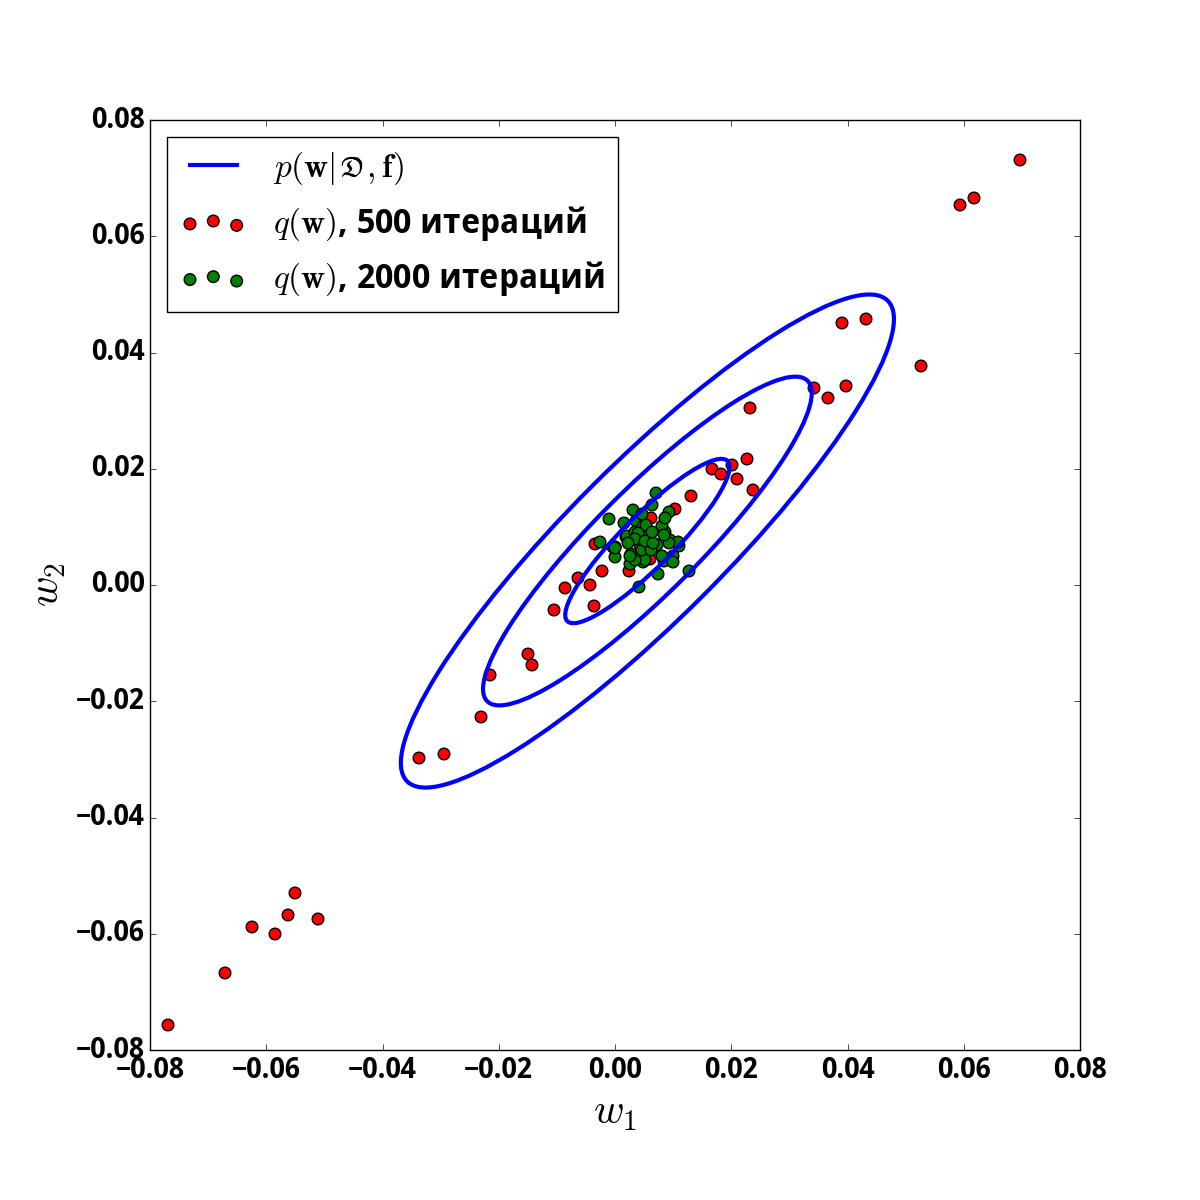
\includegraphics[width=0.52\textwidth]{./slide_plots/sgd_estimate.png}}
\end{figure}

\columnbreak


\begin{figure}
{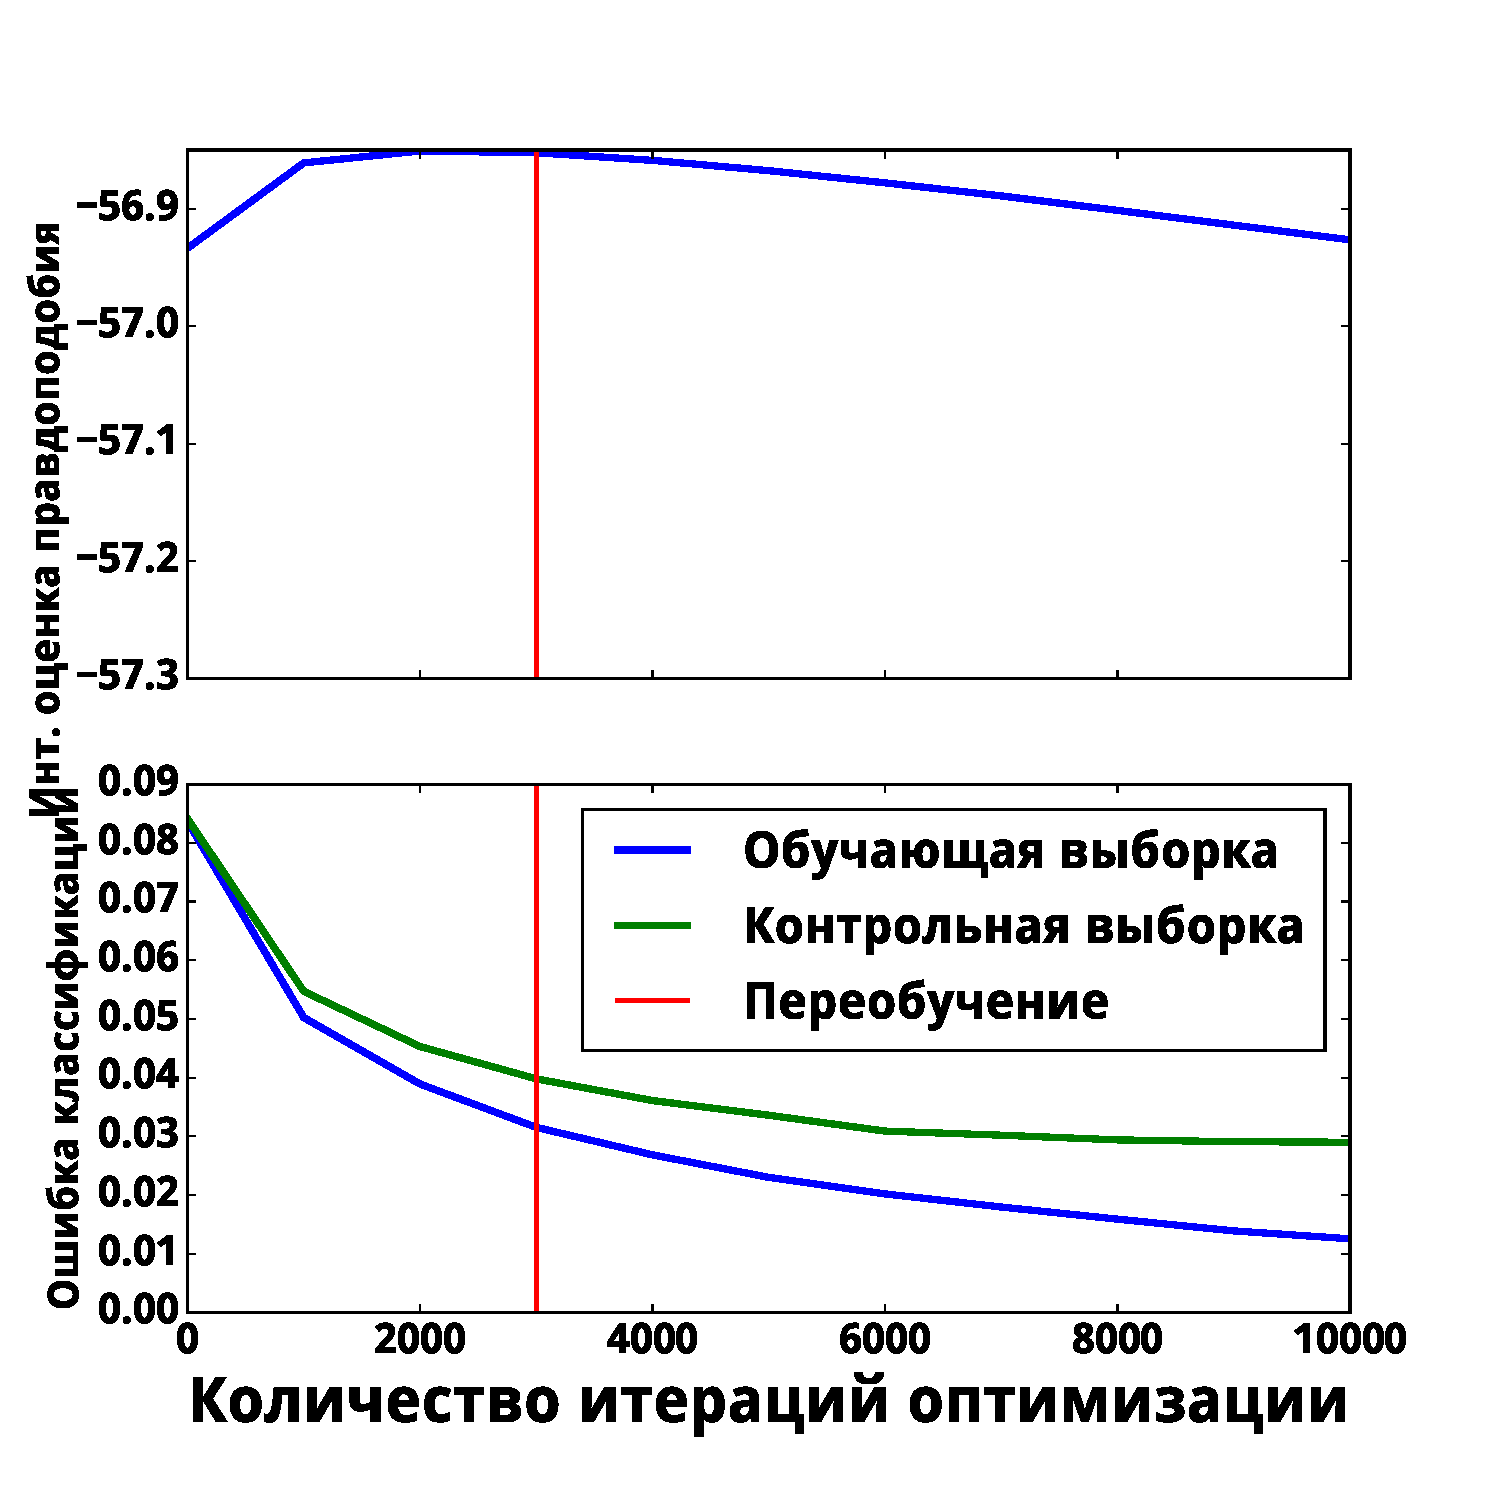
\includegraphics[width=0.52\textwidth]{./slide_plots/sgd_show.pdf}}
\end{figure}
\end{multicols}
\end{frame}








\begin{frame}{Оптимизация гиперпараметров: пример}
\begin{multicols}{2}
\begin{figure}[h]
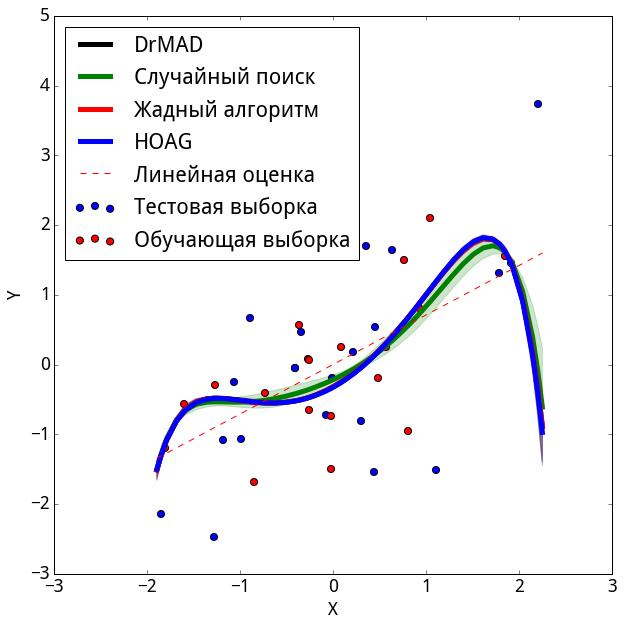
\includegraphics[width=0.4\textwidth]{./slide_plots/poly_cv.png}
\caption*{Кросс-Валидация}
\end{figure}

\begin{figure}[h]
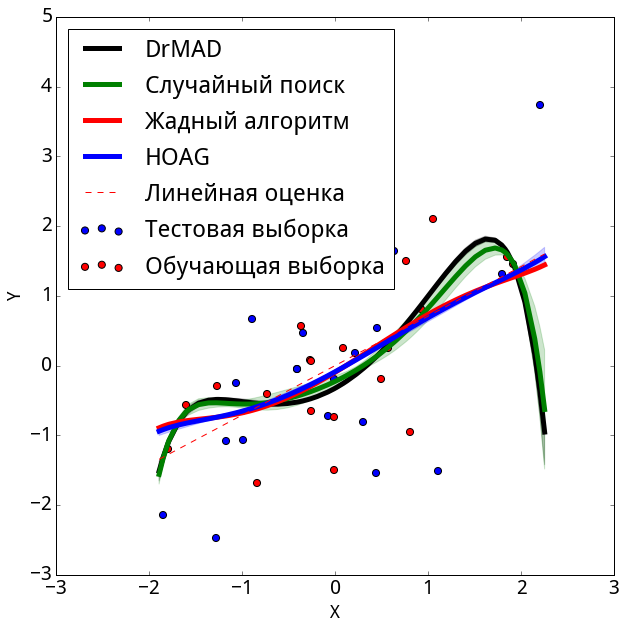
\includegraphics[width=0.4\textwidth]{./slide_plots/poly_var.png}
\caption*{Вариационная оценка}
\end{figure}
\end{multicols}

\end{frame}






\begin{frame}{Оптимизация правдоподобия модели}

\begin{block}{Теорема.}
Пусть $c_\text{reg} > 0, m \gg 0, \frac{m}{c_\text{reg}} \in \mathbb{N}.$ \\Тогда оптимизация функции \[L = 
\textcolor{blue}{\mathsf{E}_q \text{log}~{p(\mathbf{y} | \mathbf{X}, \mathbf{W}, \boldsymbol{\Gamma}, \mathbf{A}^{-1}, c_{\text{temp}})}} -\]\[- \textcolor{red}{c_\text{reg}\text{D}_{KL}(p(\mathbf{w}, \boldsymbol{\Gamma} |\mathbf{A}^{-1}, \mathbf{m}, c_{\text{temp}}) || q(\mathbf{W}), q(\boldsymbol{\Gamma}))}\] эквивалентна минимизации ожидаемой дивергенции $\mathsf{E}_{\hat{\mathbf{X}}, \hat{\mathbf{y}}\sim p(\mathbf{X}, \mathbf{y})}\text{D}_{KL}(q||p(\mathbf{w}, \boldsymbol{\Gamma} | \hat{\mathbf{X}}, \hat{\mathbf{y}})),$ где $\hat{\mathbf{X}}, \hat{\mathbf{y}}$ --- случайные подвыборки мощностью $\frac{m}{c_\text{reg}}$ из генеральной совопкупности.
\end{block}


\end{frame}

\begin{frame}{Параметрическая сложность}
\begin{block}{Определение}
Параметрической сложностью модели назовем минимальную дивергенцию между априорным и вариационным распределением:
\[
    C_p = \min_{\mathbf{h}} D_\text{KL}(q||p(\mathbf{W}, \boldsymbol{\Gamma}|c_\text{temp})).
\]
\end{block}
\begin{block}{Вариационное удаление параметров модели}
Будем удалять параметры с наибольшей относительной плотностью:
\[
\rho(w) = \frac{q(0)}{q(w)} = \text{exp}\left(-\frac{\mu^2}{\sigma^2}\right).
\]
\end{block}
\begin{block}{Теорема}
При устремлении параметрической сложности модели к нулю относительная плотность параметров модели стремится к единице:
\[
    C_p \to 0 => \boldsymbol{\rho}(\mathbf{W}) \to 1.
\]
\end{block}


%proof:
% из неравенства пинксера следует, что рано или поздно q(w) будет почти как p(w)
% у апроирного распределения мода в единице, поэтому относительная плотность будет равна 1.
\end{frame}



\begin{frame}{Оптимизация параметрической сложности}
\small
%
\begin{block}{Теорема}
Пусть $c_{\text{train}} = c_{\text{prior}} = 1, c_{\text{comb}} = 0$.
Тогда предел оптимизации
\[
\lim_{c_\text{reg} \to \infty} \lim_{\eta \to \infty}   T^\eta\bigl(Q, \mathbf{h}, T^\eta(L, \boldsymbol{\theta}_0, \mathbf{h})\bigr)
\]  
доставляет минимум параметрической сложности. 
Существует компактная область $\hat{U} \subset  U(\mathbf{0})$, такая что для любой точки $\boldsymbol{\theta}_0 \in \hat{U}$ предел данной оптимизации доставляет нулевую параметрическую сложность: $C_p = 0$.
\end{block}
% proof

% 1. Если посмотреть исходную оптимизацию (к которой стремится наша оптимизация), то это C1*Dkl - loss. Ничего не поменяется, если делить эту оптимизацию на (c1+1)
% 2. Если при этом устремить c1 > infty, то получим что коэффициент при loss стремится к нулю. Тут надо более аккуратно, но думаю здесь все ок
% 3. Рассмотрим отношение L(q = prior, m- произвольное)/L(q!=prior). Он стремится к нулю
% 4. По определению предела в некоторой окрестности эта штука тоже лежит в окрестности нуля. (скорее всего с одной стороны как непрерывная функция)
% 5. То есть в некоторой окрестности q=prior является экстремумом, при этом функция все еще непрерывная
% 6. Заметим, что для некоторой окрестности он является эктсреммумо для любой функции вида L-C*DKL, где C>0
% 6. нужно еще что-то с областью сделать




\begin{block}{Теорема}

Пусть $c_{\text{train}} = 1, c_{\text{comb}} = 0$.
Пусть  $\mathbf{f}_1, \mathbf{f}_2$ --- результаты градиентной оптимизации при разных значениях гиперпараметров $c_{\text{prior}}^1,c_{\text{prior}}^2, c_{\text{prior}}^1<c_{\text{prior}}^2$, полученных при начальном значении вариационных параметров $\boldsymbol{\theta}_0$ и гиперпараметров $\mathbf{h}_0$.
Пусть $\boldsymbol{\theta}_0, \mathbf{h}_0$ принадлежат области  $U$, в которой соответствующие функции $L$ и $Q$ являются локально-выпуклыми.
Тогда:
\[
    C_p(\mathbf{f}_1) - C_p(\mathbf{f}_2)  \geq c_\text{reg}(c_\text{reg} - c_\text{prior}^1)\text{sup}_{\boldsymbol{\theta}, \mathbf{h} \in U}|\nabla^2_{\boldsymbol{\theta}, \mathbf{h}} D_{KL}(q|p) (\nabla^2_{\boldsymbol{\theta}} L)^{-1}   \nabla_{\boldsymbol{\theta}} D_{KL}(q|p))|.
\]
\end{block}
% 1. Заметим, что покомпонентная проекция выпулкых функций - выпукла (по определению вроде). поэтому L и Q можно рассматривать как большие мета-функции.
% 2. По условиям:  L_1(q1) - c_1 DKL(q1) = max, L_2 - c_2 DKL(q_2) = max.
% 3. L_1(q1) - c_1 DKL(q1) - L_2(q2)  + c_1 DKL(q2) >= 0
%    L_2(q2) - c_2 DKL(q2) - L_1(q1) +  c_2 DKL(q1) >= 0
% 4. Складываем
%    c_1 DKL(q2) - c_2DKL(q2) >= c1 DKL(q1) - c2 DKL(q1), DKL (q2) <= DKL(q1)
% 5. Заметим, что это DKL и есть параметрической сложностью.
% Пусть существует h': DKL(q|h')<DKL(q|h).
% Так как L не зависит от h, то получается что L-DKL|h' > L-DKL|h, противоречие.
\end{frame}


\begin{frame}{Структурная сложность}
\footnotesize
\begin{block}{Определение}
Структурной сложностью $C_s$ модели назовем энтропию структур $\boldsymbol{\Gamma}$, полученных из вариационного распределения $q$:
\[
    C_s = -\mathsf{E}_q \mathsf{E}_\Gamma \text{log} p_{\boldsymbol{\Gamma}}.
\]
\end{block}

\begin{block}{Теорема}
Пусть задано априорное распределение на структуре: $$p(\boldsymbol{\gamma}_{i,j}) =  \lim_{c_{\text{temp}} \to 0} \mathcal{GS}(c_{\text{temp}}).$$
Пусть $c_{\text{reg}} >0, c_{\text{train}} >0, c_{\text{prior}}>0, c_{\text{comb}}=0$, $\mathbf{f}$ --- глобальный оптимум задачи оптимизации.
Тогда 
$
    C_s(\mathbf{f}) = 0.
$
\end{block}

\begin{block}{}
Пусть $$p(\boldsymbol{\gamma}_{i,j}) =  \lim_{c_{\text{temp}} \to \infty} \mathcal{GS}(c_{\text{temp}}).$$
Тогда структурная сложность глобального оптимума $\mathbf{f}$ равняется максимуму:
\[
    C_s(\mathbf{f}) = \mathsf{E}\text{log}\mathcal{U}.
\]
\end{block}

% NB: https://stats.stackexchange.com/questions/69125/is-it-possible-to-apply-kl-divergence-between-discrete-and-continuous-distributi, 2nd answer
% 1.Если аккуратно расписать, по stackoverflow, то получается то что и нужно
%  Для любого q, отличающегося от дискретного мы получим D_KL = inf. Итого, q - дискретно.
% 2. Поскольку у нас теперь распределение q дискретно - переберем все варианты и найдем ту позицию на вершинах симплексов, которая даст нам максимум L + DKL(q(W)).
% 3. Выберем эту вершину и сделаем p_Г = q_Г. Тогда D_KL(Г) = 0, а остальная часть достигает максимума. Итого получаем глобальный максимум
% 4. Поскольку вся фигня сконцентрирована на одно вершине, E_q = 0.

\end{frame}
\begin{frame}{Оптимизация структурной сложности}
\begin{block}{Теорема}

Пусть $c_{\text{train}} >0$, $\boldsymbol{\theta}_1, \boldsymbol{\theta}_2$ --- вариационные параметры, такие что $\boldsymbol{\theta}_1$ лежит внутри произведения симплексов структуры, $\boldsymbol{\theta}_2$ --- на вершинах симплексов.
Тогда \[
\lim_{c_\text{temp} \to 0} \frac{L(\boldsymbol{\theta}_2)}{L(\boldsymbol{\theta}_1)} \to 0.
\]
\end{block}
\begin{block}{Теорема}

Пусть $c_{\text{train}} >0$, $\boldsymbol{\theta}_1, \boldsymbol{\theta}_2$ --- вариационные параметры, такие что $\boldsymbol{\theta}_1$ лежит внутри произведения симплексов структуры, $\boldsymbol{\theta}_2$ --- в центре симплексов.
Тогда \[
\lim_{c_\text{temp} \to \infty} \frac{L(\boldsymbol{\theta}_2)}{L(\boldsymbol{\theta}_1)} \to 0.
\]
\end{block}
\end{frame}

\iffalse
\begin{frame}{Полный перебор: TODO}
\small
Пусть для каждого ребра $(i,j)$ семейства моделей $\mathfrak{F}$ априорное распределение $$p(\boldsymbol{\gamma}_{i,j}) =  lim_{c_{\text{temp}} \to 0} \mathcal{GS}(c_{\text{temp}}).$$

Рассмотрим последовательность $\mathbf{P}$, состоящую из $N = \prod_{(j,k) \in E} K_{j,k}$ моделей, полученных в ходе оптимизаций вида:
$$f_1 \in F(c_{\text{reg}}, 0, 0, \varnothing, c_{\text{comb}},  c_{\text{temp}}),$$
$$f_2 \in F(c_{\text{reg}}, 0, 0, \{q_1(\boldsymbol{\Gamma})\},  c_{\text{comb}},  c_{\text{temp}}),$$
$$f_3 \in F(c_{\text{reg}}, 0, 0, \{q_1(\boldsymbol{\Gamma}), q_2(\boldsymbol{\Gamma})\},  c_{\text{comb}},  c_{\text{temp}}),$$
где $C_{\text{reg}} > 0,  c_{\text{comb}}>0$.


\begin{block}{Теорема}
Вариационные распределения $q_{\boldsymbol{\Gamma}}$ структур  последовательности $\mathbf{P}$ вырождаются в распределения вида $\delta(\hat{\mathbf{m}})$, где $\hat{\mathbf{m}}$ --- точка на декартовом произведении вершин симплексов структуры модели.

Последовательность соответствует полному перебору структуры $\boldsymbol{\Gamma}$.
\end{block}
\end{frame}
\fi

\begin{frame}{Результаты, выносимые на защиту}
\begin{enumerate}
\item Предложен метод выбора модели наиболее правдоподобной структуры, обобщающий ранее описанные алгоритмы оптимизации:
\begin{itemize}
\item оптимизация правдоподобия;
\item последовательное увеличение сложности модели;
\item последовательное снижение сложности модели;
\item полный перебор вариантов структуры модели.
\end{itemize}

\item Предложен алгоритм оптимизации параметров, гиперпараметров и структурных
параметров моделей глубокого обучения.

\item Проведено исследование свойств алгоритмов выбора модели при различных значениях мета-параметров.

\item Проведен вычислительный эксперимент, иллюстрирующий работу предложенного метода.

\end{enumerate}
\end{frame}



\begin{frame}{Список работ автора по теме диссертации}
\tiny
\textbf{Публикации ВАК}
\begin{enumerate}
\item Бахтеев О.Ю., Попова М.С., Стрижов В.В. Системы и средства глубокого обучения в задачах классификации. // Системы и средства информатики. 2016. № 26.2. С. 4-22.
\item Бахтеев О.Ю., Стрижов В.В. Выбор моделей глубокого обучения субоптимальной сложности. // Автоматика и телемеханика. 2018. №8. С. 129-147.
\item Огальцов А.В., Бахтеев О.Ю. Автоматическое извлечение метаданных из научных PDF-документов. // Информатика и её применения. 2018.
\item Смердов А.Н., Бахтеев О.Ю., Стрижов В.В. Выбор оптимальной модели рекуррентной сети в задачах поиска парафраза. // Информатика и ее применения. 2019.
\item Грабовой А.В., Бахтеев О.Ю., Стрижов В.В. Определение релевантности параметров нейросети. // Информатика и её применения. 2019.
\end{enumerate}
\textbf{Выступления с докладом}
\begin{enumerate}
\item ``Восстановление панельной матрицы и ранжирующей модели в разнородных шкалах'', Всероссийская конеренция <<57-я научная конеренция МФТИ>>, 2014.
\item ``A monolingual approach to detection of text reuse in Russian-English collection'', Международная конференция <<Artificial Intelligence and Natural Language Conference>>, 2015.
\item ``Выбор модели глубокого обучения субоптимальной сложности с использованием вариационной оценки правдоподобия'', Международная конференция <<Интеллектуализация обработки информации>>, 2016.
\item ``Author Masking using Sequence-to-Sequence Models'', Международная конференция <<Conference and Labs of the Evaluation Forum>>, 2017.
\item ``Градиентные методы оптимизации гиперпараметров моделей глубокого обучения'', Всероссийская конференция <<Математические методы распознавания образов ММРО>>, 2017.
\item ``Детектирование переводных заимствований в текстах научных статей из журналов, входящих в РИНЦ'', Всероссийская конференция <<Математические методы распознавания образов ММРО>>, 2017.
\item ``Байесовский выбор наиболее правдоподобной структуры модели глубокого обучения'', Международная конференция <<Интеллектуализация обработки информации>>, 2018.
\end{enumerate}
\end{frame}





\end{document}
